%% IEEE Access version, generated by jr/build_access.py from paper/main.tex. Edit paper/main_body.tex
%% and rebuild; do not edit this file by hand unless you stop using the build.
\documentclass{ieeeaccess}
\usepackage{cite}
\usepackage{amsmath,amssymb,amsfonts}
\usepackage{amsthm}
\usepackage{graphicx}
\usepackage{textcomp}
\usepackage{booktabs}
\usepackage{multirow}
\usepackage{url}
\def\UrlBreaks{\do\/\do-\do.}

\usepackage{bm}
\makeatletter
\AtBeginDocument{\DeclareMathVersion{bold}
\SetSymbolFont{operators}{bold}{T1}{times}{b}{n}
\SetSymbolFont{NewLetters}{bold}{T1}{times}{b}{it}
\SetMathAlphabet{\mathrm}{bold}{T1}{times}{b}{n}
\SetMathAlphabet{\mathit}{bold}{T1}{times}{b}{it}
\SetMathAlphabet{\mathbf}{bold}{T1}{times}{b}{n}
\SetMathAlphabet{\mathtt}{bold}{OT1}{pcr}{b}{n}
\SetSymbolFont{symbols}{bold}{OMS}{cmsy}{b}{n}
\renewcommand\boldmath{\@nomath\boldmath\mathversion{bold}}}
\makeatother

\newtheorem{proposition}{Proposition}
\newtheorem{definition}{Definition}

%% Every number in the text and tables, generated from the result files.
\newcommand{\PiZero}{0.867}
\newcommand{\NegAll}{496}
\newcommand{\NegStruct}{430}
\newcommand{\AucNonempty}{0.885}
\newcommand{\AucAll}{0.985}
\newcommand{\AucPred}{0.985}
\newcommand{\AZero}{1.000}
\newcommand{\Inflation}{0.099}
\newcommand{\TrainPrev}{0.41}
\newcommand{\TrainRatio}{1.4}
\newcommand{\ExtProjects}{8}
\newcommand{\PrevMin}{0.07}
\newcommand{\PrevMax}{0.59}
\newcommand{\RatioMin}{13}
\newcommand{\RatioMax}{0.7}
\newcommand{\SensMin}{0.00}
\newcommand{\SensMax}{0.86}
\newcommand{\SpearmanPS}{0.93}
\newcommand{\CarryMedian}{0.67}
\newcommand{\Qhat}{0.33}
\newcommand{\PSpillThree}{0.963}
\newcommand{\NonemptySpill}{90.1}
\newcommand{\MedianIssues}{6}
\newcommand{\OverlapShare}{57}
\newcommand{\NoFallbackTest}{356}
\newcommand{\FallbackMean}{12.9}
\newcommand{\Rhat}{0.18}
\newcommand{\DispRatio}{4.5}
\newcommand{\LRstat}{2,181}
\newcommand{\NProjSprints}{36}
\newcommand{\NProjThirty}{32}
\newcommand{\NProjExport}{29}
\newcommand{\NProj}{26}
\newcommand{\NSprints}{3,676}
\newcommand{\NNonempty}{2,409}
\newcommand{\SprintMin}{35}
\newcommand{\SprintMax}{557}
\newcommand{\SprintMed}{102}
\newcommand{\DateFrom}{February 2012}
\newcommand{\DateTo}{October 2020}
\newcommand{\TestAll}{1,118}
\newcommand{\TestNonempty}{734}
\newcommand{\NegSp}{73}
\newcommand{\NegSs}{110}
\newcommand{\CarryMedPct}{67}
\newcommand{\PosSs}{82}
\newcommand{\PosSm}{49}
\newcommand{\PosSp}{90}
\newcommand{\DevProj}{7}
\newcommand{\DevSprints}{2,138}
\newcommand{\ConfProj}{19}
\newcommand{\NExcluded}{3}
\newcommand{\UnrecA}{69}
\newcommand{\UnrecB}{57}
\newcommand{\UnrecC}{56}
\newcommand{\UnrecOtherMax}{0.7}
\newcommand{\FullNothingPct}{31}
\newcommand{\FullSprints}{4,235}
\newcommand{\CleanNothingPct}{26}
\newcommand{\dPTNewLc}{0.001}
\newcommand{\cPTNewLc}{[$-$0.013, 0.012]}
\newcommand{\dPTHistLc}{0.043}
\newcommand{\cPTHistLc}{[$-$0.013, 0.093]}
\newcommand{\dPTStrLc}{0.042}
\newcommand{\cPTStrLc}{[$-$0.020, 0.102]}
\newcommand{\dPTNewSl}{$-$0.006}
\newcommand{\cPTNewSl}{[$-$0.016, 0.000]}
\newcommand{\dPTHistSl}{0.045}
\newcommand{\cPTHistSl}{[$-$0.020, 0.101]}
\newcommand{\dPTStrSl}{0.051}
\newcommand{\cPTStrSl}{[$-$0.014, 0.114]}
\newcommand{\dPTNewSp}{0.037}
\newcommand{\cPTNewSp}{[0.022, 0.056]}
\newcommand{\dPTHistSp}{0.034}
\newcommand{\cPTHistSp}{[$-$0.005, 0.082]}
\newcommand{\dPTStrSp}{$-$0.003}
\newcommand{\cPTStrSp}{[$-$0.051, 0.043]}
\newcommand{\dPTNewSs}{0.017}
\newcommand{\cPTNewSs}{[$-$0.008, 0.048]}
\newcommand{\dPTHistSs}{0.088}
\newcommand{\cPTHistSs}{[0.018, 0.161]}
\newcommand{\dPTStrSs}{0.071}
\newcommand{\cPTStrSs}{[0.001, 0.141]}
\newcommand{\dPTNewSc}{0.026}
\newcommand{\cPTNewSc}{[$-$0.028, 0.069]}
\newcommand{\dPTHistSc}{0.063}
\newcommand{\cPTHistSc}{[$-$0.056, 0.207]}
\newcommand{\dPTStrSc}{0.037}
\newcommand{\cPTStrSc}{[$-$0.067, 0.172]}
\newcommand{\dPTNewSt}{0.030}
\newcommand{\cPTNewSt}{[0.018, 0.051]}
\newcommand{\dPTHistSt}{0.035}
\newcommand{\cPTHistSt}{[$-$0.036, 0.113]}
\newcommand{\dPTStrSt}{0.005}
\newcommand{\cPTStrSt}{[$-$0.074, 0.075]}
\newcommand{\dPTNewSf}{0.030}
\newcommand{\cPTNewSf}{[$-$0.001, 0.064]}
\newcommand{\dPTHistSf}{0.103}
\newcommand{\cPTHistSf}{[0.024, 0.176]}
\newcommand{\dPTStrSf}{0.072}
\newcommand{\cPTStrSf}{[$-$0.009, 0.140]}
\newcommand{\dPTNewSh}{0.063}
\newcommand{\cPTNewSh}{[0.021, 0.098]}
\newcommand{\dPTHistSh}{0.065}
\newcommand{\cPTHistSh}{[$-$0.033, 0.173]}
\newcommand{\dPTStrSh}{0.002}
\newcommand{\cPTStrSh}{[$-$0.108, 0.128]}
\newcommand{\dPTNewSm}{0.037}
\newcommand{\cPTNewSm}{[0.010, 0.061]}
\newcommand{\dPTHistSm}{0.141}
\newcommand{\cPTHistSm}{[0.065, 0.206]}
\newcommand{\dPTStrSm}{0.104}
\newcommand{\cPTStrSm}{[0.037, 0.165]}
\newcommand{\dPLNewLc}{$-$0.003}
\newcommand{\cPLNewLc}{[$-$0.009, 0.003]}
\newcommand{\dPLHistLc}{0.077}
\newcommand{\cPLHistLc}{[0.037, 0.115]}
\newcommand{\dPLStrLc}{0.080}
\newcommand{\cPLStrLc}{[0.036, 0.117]}
\newcommand{\dPLNewSl}{$-$0.008}
\newcommand{\cPLNewSl}{[$-$0.016, 0.000]}
\newcommand{\dPLHistSl}{0.024}
\newcommand{\cPLHistSl}{[$-$0.005, 0.058]}
\newcommand{\dPLStrSl}{0.033}
\newcommand{\cPLStrSl}{[0.003, 0.068]}
\newcommand{\dPLNewSp}{0.015}
\newcommand{\cPLNewSp}{[0.003, 0.034]}
\newcommand{\dPLHistSp}{0.031}
\newcommand{\cPLHistSp}{[0.003, 0.061]}
\newcommand{\dPLStrSp}{0.016}
\newcommand{\cPLStrSp}{[$-$0.015, 0.043]}
\newcommand{\dPLNewSs}{0.024}
\newcommand{\cPLNewSs}{[0.005, 0.047]}
\newcommand{\dPLHistSs}{0.138}
\newcommand{\cPLHistSs}{[0.088, 0.183]}
\newcommand{\dPLStrSs}{0.114}
\newcommand{\cPLStrSs}{[0.056, 0.161]}
\newcommand{\dPLNewSc}{0.024}
\newcommand{\cPLNewSc}{[$-$0.011, 0.071]}
\newcommand{\dPLHistSc}{0.012}
\newcommand{\cPLHistSc}{[$-$0.047, 0.097]}
\newcommand{\dPLStrSc}{$-$0.012}
\newcommand{\cPLStrSc}{[$-$0.058, 0.049]}
\newcommand{\dPLNewSt}{0.029}
\newcommand{\cPLNewSt}{[0.014, 0.050]}
\newcommand{\dPLHistSt}{0.108}
\newcommand{\cPLHistSt}{[0.049, 0.165]}
\newcommand{\dPLStrSt}{0.079}
\newcommand{\cPLStrSt}{[0.014, 0.142]}
\newcommand{\dPLNewSf}{0.031}
\newcommand{\cPLNewSf}{[0.012, 0.047]}
\newcommand{\dPLHistSf}{0.194}
\newcommand{\cPLHistSf}{[0.113, 0.271]}
\newcommand{\dPLStrSf}{0.163}
\newcommand{\cPLStrSf}{[0.080, 0.234]}
\newcommand{\dPLNewSh}{0.024}
\newcommand{\cPLNewSh}{[$-$0.012, 0.065]}
\newcommand{\dPLHistSh}{0.005}
\newcommand{\cPLHistSh}{[$-$0.046, 0.089]}
\newcommand{\dPLStrSh}{$-$0.019}
\newcommand{\cPLStrSh}{[$-$0.065, 0.052]}
\newcommand{\dPLNewSm}{0.029}
\newcommand{\cPLNewSm}{[0.009, 0.049]}
\newcommand{\dPLHistSm}{0.165}
\newcommand{\cPLHistSm}{[0.116, 0.215]}
\newcommand{\dPLStrSm}{0.136}
\newcommand{\cPLStrSm}{[0.090, 0.196]}
\newcommand{\dPFNewSp}{0.041}
\newcommand{\cPFNewSp}{[0.015, 0.064]}
\newcommand{\dPFHistSp}{0.069}
\newcommand{\cPFHistSp}{[0.013, 0.120]}
\newcommand{\dPFStrSp}{0.028}
\newcommand{\cPFStrSp}{[$-$0.036, 0.082]}
\newcommand{\dPFNewSs}{0.029}
\newcommand{\cPFNewSs}{[0.002, 0.058]}
\newcommand{\dPFHistSs}{0.125}
\newcommand{\cPFHistSs}{[0.025, 0.215]}
\newcommand{\dPFStrSs}{0.096}
\newcommand{\cPFStrSs}{[0.002, 0.183]}
\newcommand{\dPFNewSc}{0.022}
\newcommand{\cPFNewSc}{[$-$0.052, 0.117]}
\newcommand{\dPFHistSc}{0.162}
\newcommand{\cPFHistSc}{[$-$0.041, 0.280]}
\newcommand{\dPFStrSc}{0.140}
\newcommand{\cPFStrSc}{[$-$0.108, 0.279]}
\newcommand{\dITWkSpA}{0.131}
\newcommand{\cITWkSpA}{[0.077, 0.196]}
\newcommand{\dITChSpA}{0.031}
\newcommand{\cITChSpA}{[$-$0.002, 0.067]}
\newcommand{\dITAddSpA}{$-$0.002}
\newcommand{\cITAddSpA}{[$-$0.006, 0.003]}
\newcommand{\dITWsSpA}{$-$0.046}
\newcommand{\cITWsSpA}{[$-$0.116, 0.014]}
\newcommand{\dITCsSpA}{0.054}
\newcommand{\cITCsSpA}{[0.015, 0.097]}
\newcommand{\dITCtxSpA}{0.012}
\newcommand{\cITCtxSpA}{[$-$0.013, 0.043]}
\newcommand{\dITProgSpA}{0.018}
\newcommand{\cITProgSpA}{[$-$0.008, 0.048]}
\newcommand{\dITWkSpB}{0.194}
\newcommand{\cITWkSpB}{[0.109, 0.272]}
\newcommand{\dITChSpB}{0.034}
\newcommand{\cITChSpB}{[0.000, 0.078]}
\newcommand{\dITAddSpB}{0.000}
\newcommand{\cITAddSpB}{[$-$0.006, 0.004]}
\newcommand{\dITWsSpB}{$-$0.090}
\newcommand{\cITWsSpB}{[$-$0.170, $-$0.019]}
\newcommand{\dITCsSpB}{0.069}
\newcommand{\cITCsSpB}{[0.036, 0.107]}
\newcommand{\dITCtxSpB}{0.007}
\newcommand{\cITCtxSpB}{[$-$0.014, 0.032]}
\newcommand{\dITProgSpB}{0.027}
\newcommand{\cITProgSpB}{[$-$0.004, 0.061]}
\newcommand{\dITWkLcA}{0.144}
\newcommand{\cITWkLcA}{[0.074, 0.214]}
\newcommand{\dITChLcA}{0.051}
\newcommand{\cITChLcA}{[$-$0.010, 0.125]}
\newcommand{\dITAddLcA}{0.001}
\newcommand{\cITAddLcA}{[$-$0.009, 0.010]}
\newcommand{\dITWsLcA}{$-$0.107}
\newcommand{\cITWsLcA}{[$-$0.164, $-$0.040]}
\newcommand{\dITCsLcA}{$-$0.013}
\newcommand{\cITCsLcA}{[$-$0.094, 0.049]}
\newcommand{\dITCtxLcA}{0.059}
\newcommand{\cITCtxLcA}{[$-$0.001, 0.125]}
\newcommand{\dITProgLcA}{$-$0.008}
\newcommand{\cITProgLcA}{[$-$0.022, 0.008]}
\newcommand{\dITWkLcB}{0.098}
\newcommand{\cITWkLcB}{[0.007, 0.184]}
\newcommand{\dITChLcB}{0.053}
\newcommand{\cITChLcB}{[$-$0.013, 0.125]}
\newcommand{\dITAddLcB}{0.004}
\newcommand{\cITAddLcB}{[$-$0.003, 0.012]}
\newcommand{\dITWsLcB}{$-$0.043}
\newcommand{\cITWsLcB}{[$-$0.105, 0.025]}
\newcommand{\dITCsLcB}{0.002}
\newcommand{\cITCsLcB}{[$-$0.062, 0.060]}
\newcommand{\dITCtxLcB}{0.063}
\newcommand{\cITCtxLcB}{[$-$0.001, 0.135]}
\newcommand{\dITProgLcB}{$-$0.011}
\newcommand{\cITProgLcB}{[$-$0.023, 0.003]}
\newcommand{\dITWkSsA}{0.179}
\newcommand{\cITWkSsA}{[0.108, 0.256]}
\newcommand{\dITChSsA}{0.049}
\newcommand{\cITChSsA}{[0.000, 0.111]}
\newcommand{\dITAddSsA}{$-$0.002}
\newcommand{\cITAddSsA}{[$-$0.008, 0.004]}
\newcommand{\dITWsSsA}{$-$0.030}
\newcommand{\cITWsSsA}{[$-$0.137, 0.055]}
\newcommand{\dITCsSsA}{0.099}
\newcommand{\cITCsSsA}{[0.024, 0.171]}
\newcommand{\dITCtxSsA}{0.034}
\newcommand{\cITCtxSsA}{[$-$0.011, 0.093]}
\newcommand{\dITProgSsA}{0.016}
\newcommand{\cITProgSsA}{[$-$0.018, 0.048]}
\newcommand{\dITWkSsB}{0.178}
\newcommand{\cITWkSsB}{[0.083, 0.261]}
\newcommand{\dITChSsB}{0.053}
\newcommand{\cITChSsB}{[0.000, 0.117]}
\newcommand{\dITAddSsB}{0.000}
\newcommand{\cITAddSsB}{[$-$0.006, 0.005]}
\newcommand{\dITWsSsB}{0.019}
\newcommand{\cITWsSsB}{[$-$0.069, 0.117]}
\newcommand{\dITCsSsB}{0.145}
\newcommand{\cITCsSsB}{[0.077, 0.216]}
\newcommand{\dITCtxSsB}{0.018}
\newcommand{\cITCtxSsB}{[$-$0.021, 0.070]}
\newcommand{\dITProgSsB}{0.034}
\newcommand{\cITProgSsB}{[0.005, 0.069]}
\newcommand{\dITWkSlA}{0.169}
\newcommand{\cITWkSlA}{[0.072, 0.274]}
\newcommand{\dITChSlA}{0.067}
\newcommand{\cITChSlA}{[$-$0.008, 0.138]}
\newcommand{\dITAddSlA}{$-$0.003}
\newcommand{\cITAddSlA}{[$-$0.014, 0.008]}
\newcommand{\dITWsSlA}{$-$0.111}
\newcommand{\cITWsSlA}{[$-$0.186, $-$0.050]}
\newcommand{\dITCsSlA}{$-$0.009}
\newcommand{\cITCsSlA}{[$-$0.076, 0.042]}
\newcommand{\dITCtxSlA}{0.038}
\newcommand{\cITCtxSlA}{[$-$0.029, 0.105]}
\newcommand{\dITProgSlA}{0.029}
\newcommand{\cITProgSlA}{[0.002, 0.055]}
\newcommand{\dITWkSlB}{0.149}
\newcommand{\cITWkSlB}{[0.067, 0.243]}
\newcommand{\dITChSlB}{0.093}
\newcommand{\cITChSlB}{[0.007, 0.193]}
\newcommand{\dITAddSlB}{$-$0.007}
\newcommand{\cITAddSlB}{[$-$0.018, 0.007]}
\newcommand{\dITWsSlB}{$-$0.068}
\newcommand{\cITWsSlB}{[$-$0.143, $-$0.004]}
\newcommand{\dITCsSlB}{$-$0.011}
\newcommand{\cITCsSlB}{[$-$0.098, 0.056]}
\newcommand{\dITCtxSlB}{0.099}
\newcommand{\cITCtxSlB}{[0.011, 0.192]}
\newcommand{\dITProgSlB}{$-$0.006}
\newcommand{\cITProgSlB}{[$-$0.042, 0.028]}
\newcommand{\dILWkSpA}{0.188}
\newcommand{\cILWkSpA}{[0.152, 0.235]}
\newcommand{\dILChSpA}{0.022}
\newcommand{\cILChSpA}{[0.004, 0.043]}
\newcommand{\dILAddSpA}{$-$0.001}
\newcommand{\cILAddSpA}{[$-$0.005, 0.001]}
\newcommand{\dILWsSpA}{$-$0.106}
\newcommand{\cILWsSpA}{[$-$0.180, $-$0.055]}
\newcommand{\dILCsSpA}{0.059}
\newcommand{\cILCsSpA}{[0.029, 0.091]}
\newcommand{\dILCtxSpA}{0.005}
\newcommand{\cILCtxSpA}{[$-$0.006, 0.019]}
\newcommand{\dILProgSpA}{0.017}
\newcommand{\cILProgSpA}{[0.002, 0.031]}
\newcommand{\dILWkSpB}{0.165}
\newcommand{\cILWkSpB}{[0.120, 0.222]}
\newcommand{\dILChSpB}{0.023}
\newcommand{\cILChSpB}{[0.003, 0.044]}
\newcommand{\dILAddSpB}{0.000}
\newcommand{\cILAddSpB}{[$-$0.004, 0.003]}
\newcommand{\dILWsSpB}{$-$0.057}
\newcommand{\cILWsSpB}{[$-$0.131, $-$0.007]}
\newcommand{\dILCsSpB}{0.085}
\newcommand{\cILCsSpB}{[0.051, 0.119]}
\newcommand{\dILCtxSpB}{0.000}
\newcommand{\cILCtxSpB}{[$-$0.009, 0.012]}
\newcommand{\dILProgSpB}{0.023}
\newcommand{\cILProgSpB}{[0.008, 0.036]}
\newcommand{\dILWkLcA}{0.182}
\newcommand{\cILWkLcA}{[0.109, 0.258]}
\newcommand{\dILChLcA}{0.056}
\newcommand{\cILChLcA}{[$-$0.021, 0.142]}
\newcommand{\dILAddLcA}{0.004}
\newcommand{\cILAddLcA}{[$-$0.004, 0.012]}
\newcommand{\dILWsLcA}{$-$0.085}
\newcommand{\cILWsLcA}{[$-$0.125, $-$0.050]}
\newcommand{\dILCsLcA}{0.041}
\newcommand{\cILCsLcA}{[$-$0.005, 0.073]}
\newcommand{\dILCtxLcA}{0.054}
\newcommand{\cILCtxLcA}{[$-$0.012, 0.123]}
\newcommand{\dILProgLcA}{0.002}
\newcommand{\cILProgLcA}{[$-$0.011, 0.024]}
\newcommand{\dILWkLcB}{0.124}
\newcommand{\cILWkLcB}{[0.045, 0.208]}
\newcommand{\dILChLcB}{0.076}
\newcommand{\cILChLcB}{[0.005, 0.157]}
\newcommand{\dILAddLcB}{0.003}
\newcommand{\cILAddLcB}{[$-$0.005, 0.010]}
\newcommand{\dILWsLcB}{$-$0.023}
\newcommand{\cILWsLcB}{[$-$0.082, 0.029]}
\newcommand{\dILCsLcB}{0.026}
\newcommand{\cILCsLcB}{[$-$0.023, 0.062]}
\newcommand{\dILCtxLcB}{0.064}
\newcommand{\cILCtxLcB}{[$-$0.007, 0.145]}
\newcommand{\dILProgLcB}{0.012}
\newcommand{\cILProgLcB}{[0.003, 0.021]}
\newcommand{\dILWkSsA}{0.206}
\newcommand{\cILWkSsA}{[0.152, 0.269]}
\newcommand{\dILChSsA}{0.070}
\newcommand{\cILChSsA}{[0.044, 0.097]}
\newcommand{\dILAddSsA}{0.002}
\newcommand{\cILAddSsA}{[$-$0.002, 0.005]}
\newcommand{\dILWsSsA}{0.013}
\newcommand{\cILWsSsA}{[$-$0.081, 0.092]}
\newcommand{\dILCsSsA}{0.149}
\newcommand{\cILCsSsA}{[0.096, 0.190]}
\newcommand{\dILCtxSsA}{0.057}
\newcommand{\cILCtxSsA}{[0.032, 0.084]}
\newcommand{\dILProgSsA}{0.012}
\newcommand{\cILProgSsA}{[$-$0.004, 0.028]}
\newcommand{\dILWkSsB}{0.162}
\newcommand{\cILWkSsB}{[0.132, 0.196]}
\newcommand{\dILChSsB}{0.061}
\newcommand{\cILChSsB}{[0.036, 0.088]}
\newcommand{\dILAddSsB}{$-$0.001}
\newcommand{\cILAddSsB}{[$-$0.003, 0.003]}
\newcommand{\dILWsSsB}{0.112}
\newcommand{\cILWsSsB}{[0.042, 0.157]}
\newcommand{\dILCsSsB}{0.213}
\newcommand{\cILCsSsB}{[0.161, 0.258]}
\newcommand{\dILCtxSsB}{0.024}
\newcommand{\cILCtxSsB}{[0.005, 0.041]}
\newcommand{\dILProgSsB}{0.037}
\newcommand{\cILProgSsB}{[0.020, 0.057]}
\newcommand{\dILWkSlA}{0.067}
\newcommand{\cILWkSlA}{[$-$0.009, 0.160]}
\newcommand{\dILChSlA}{0.022}
\newcommand{\cILChSlA}{[$-$0.030, 0.085]}
\newcommand{\dILAddSlA}{0.009}
\newcommand{\cILAddSlA}{[0.003, 0.015]}
\newcommand{\dILWsSlA}{$-$0.035}
\newcommand{\cILWsSlA}{[$-$0.137, 0.058]}
\newcommand{\dILCsSlA}{0.009}
\newcommand{\cILCsSlA}{[$-$0.048, 0.048]}
\newcommand{\dILCtxSlA}{0.032}
\newcommand{\cILCtxSlA}{[$-$0.011, 0.088]}
\newcommand{\dILProgSlA}{$-$0.011}
\newcommand{\cILProgSlA}{[$-$0.028, 0.007]}
\newcommand{\dILWkSlB}{0.067}
\newcommand{\cILWkSlB}{[0.006, 0.149]}
\newcommand{\dILChSlB}{0.028}
\newcommand{\cILChSlB}{[$-$0.024, 0.097]}
\newcommand{\dILAddSlB}{0.010}
\newcommand{\cILAddSlB}{[$-$0.003, 0.022]}
\newcommand{\dILWsSlB}{$-$0.030}
\newcommand{\cILWsSlB}{[$-$0.121, 0.046]}
\newcommand{\dILCsSlB}{0.008}
\newcommand{\cILCsSlB}{[$-$0.054, 0.048]}
\newcommand{\dILCtxSlB}{0.029}
\newcommand{\cILCtxSlB}{[$-$0.018, 0.094]}
\newcommand{\dILProgSlB}{0.000}
\newcommand{\cILProgSlB}{[$-$0.021, 0.020]}
\newcommand{\dPCNewLc}{$-$0.009}
\newcommand{\cPCNewLc}{[$-$0.025, 0.005]}
\newcommand{\dPCHistLc}{0.016}
\newcommand{\cPCHistLc}{[$-$0.050, 0.081]}
\newcommand{\dPCStrLc}{0.025}
\newcommand{\cPCStrLc}{[$-$0.049, 0.096]}
\newcommand{\dPCNewSl}{0.002}
\newcommand{\cPCNewSl}{[$-$0.006, 0.012]}
\newcommand{\dPCHistSl}{0.044}
\newcommand{\cPCHistSl}{[$-$0.009, 0.085]}
\newcommand{\dPCStrSl}{0.041}
\newcommand{\cPCStrSl}{[$-$0.012, 0.084]}
\newcommand{\dPCNewSp}{0.016}
\newcommand{\cPCNewSp}{[$-$0.016, 0.048]}
\newcommand{\dPCHistSp}{0.089}
\newcommand{\cPCHistSp}{[0.044, 0.137]}
\newcommand{\dPCStrSp}{0.073}
\newcommand{\cPCStrSp}{[0.033, 0.109]}
\newcommand{\dPCNewSs}{0.035}
\newcommand{\cPCNewSs}{[$-$0.007, 0.080]}
\newcommand{\dPCHistSs}{0.178}
\newcommand{\cPCHistSs}{[0.092, 0.256]}
\newcommand{\dPCStrSs}{0.143}
\newcommand{\cPCStrSs}{[0.042, 0.221]}
\newcommand{\dPCNewSc}{0.006}
\newcommand{\cPCNewSc}{[$-$0.044, 0.056]}
\newcommand{\dPCHistSc}{0.065}
\newcommand{\cPCHistSc}{[$-$0.105, 0.193]}
\newcommand{\dPCStrSc}{0.059}
\newcommand{\cPCStrSc}{[$-$0.136, 0.201]}
\newcommand{\dICWkSpA}{0.158}
\newcommand{\cICWkSpA}{[0.057, 0.249]}
\newcommand{\dICChSpA}{0.053}
\newcommand{\cICChSpA}{[0.007, 0.101]}
\newcommand{\dICAddSpA}{0.005}
\newcommand{\cICAddSpA}{[$-$0.005, 0.013]}
\newcommand{\dICWsSpA}{$-$0.023}
\newcommand{\cICWsSpA}{[$-$0.122, 0.081]}
\newcommand{\dICCsSpA}{0.082}
\newcommand{\cICCsSpA}{[0.028, 0.129]}
\newcommand{\dICCtxSpA}{0.033}
\newcommand{\cICCtxSpA}{[$-$0.004, 0.068]}
\newcommand{\dICProgSpA}{0.021}
\newcommand{\cICProgSpA}{[$-$0.018, 0.069]}
\newcommand{\dICWkSpB}{0.252}
\newcommand{\cICWkSpB}{[0.140, 0.366]}
\newcommand{\dICChSpB}{0.081}
\newcommand{\cICChSpB}{[0.022, 0.145]}
\newcommand{\dICAddSpB}{0.002}
\newcommand{\cICAddSpB}{[$-$0.005, 0.009]}
\newcommand{\dICWsSpB}{$-$0.057}
\newcommand{\cICWsSpB}{[$-$0.144, 0.049]}
\newcommand{\dICCsSpB}{0.114}
\newcommand{\cICCsSpB}{[0.063, 0.167]}
\newcommand{\dICCtxSpB}{0.032}
\newcommand{\cICCtxSpB}{[0.003, 0.062]}
\newcommand{\dICProgSpB}{0.048}
\newcommand{\cICProgSpB}{[$-$0.001, 0.113]}
\newcommand{\dICWkLcA}{0.154}
\newcommand{\cICWkLcA}{[0.045, 0.253]}
\newcommand{\dICChLcA}{0.032}
\newcommand{\cICChLcA}{[$-$0.028, 0.088]}
\newcommand{\dICAddLcA}{0.000}
\newcommand{\cICAddLcA}{[$-$0.013, 0.012]}
\newcommand{\dICWsLcA}{$-$0.099}
\newcommand{\cICWsLcA}{[$-$0.217, 0.016]}
\newcommand{\dICCsLcA}{0.024}
\newcommand{\cICCsLcA}{[$-$0.037, 0.075]}
\newcommand{\dICCtxLcA}{0.034}
\newcommand{\cICCtxLcA}{[$-$0.023, 0.092]}
\newcommand{\dICProgLcA}{$-$0.002}
\newcommand{\cICProgLcA}{[$-$0.030, 0.029]}
\newcommand{\dICWkLcB}{0.032}
\newcommand{\cICWkLcB}{[$-$0.058, 0.107]}
\newcommand{\dICChLcB}{0.028}
\newcommand{\cICChLcB}{[$-$0.031, 0.083]}
\newcommand{\dICAddLcB}{0.002}
\newcommand{\cICAddLcB}{[$-$0.010, 0.017]}
\newcommand{\dICWsLcB}{0.027}
\newcommand{\cICWsLcB}{[$-$0.068, 0.136]}
\newcommand{\dICCsLcB}{0.031}
\newcommand{\cICCsLcB}{[$-$0.029, 0.088]}
\newcommand{\dICCtxLcB}{0.035}
\newcommand{\cICCtxLcB}{[$-$0.018, 0.095]}
\newcommand{\dICProgLcB}{$-$0.006}
\newcommand{\cICProgLcB}{[$-$0.028, 0.014]}
\newcommand{\dICWkSsA}{0.236}
\newcommand{\cICWkSsA}{[0.173, 0.321]}
\newcommand{\dICChSsA}{0.111}
\newcommand{\cICChSsA}{[0.038, 0.209]}
\newcommand{\dICAddSsA}{$-$0.007}
\newcommand{\cICAddSsA}{[$-$0.021, 0.004]}
\newcommand{\dICWsSsA}{0.048}
\newcommand{\cICWsSsA}{[$-$0.096, 0.185]}
\newcommand{\dICCsSsA}{0.174}
\newcommand{\cICCsSsA}{[0.041, 0.286]}
\newcommand{\dICCtxSsA}{0.059}
\newcommand{\cICCtxSsA}{[$-$0.002, 0.135]}
\newcommand{\dICProgSsA}{0.052}
\newcommand{\cICProgSsA}{[0.018, 0.097]}
\newcommand{\dICWkSsB}{0.248}
\newcommand{\cICWkSsB}{[0.168, 0.300]}
\newcommand{\dICChSsB}{0.099}
\newcommand{\cICChSsB}{[0.048, 0.165]}
\newcommand{\dICAddSsB}{0.005}
\newcommand{\cICAddSsB}{[$-$0.008, 0.018]}
\newcommand{\dICWsSsB}{0.094}
\newcommand{\cICWsSsB}{[$-$0.007, 0.227]}
\newcommand{\dICCsSsB}{0.244}
\newcommand{\cICCsSsB}{[0.128, 0.357]}
\newcommand{\dICCtxSsB}{0.032}
\newcommand{\cICCtxSsB}{[0.003, 0.062]}
\newcommand{\dICProgSsB}{0.067}
\newcommand{\cICProgSsB}{[0.024, 0.122]}
\newcommand{\dICWkSlA}{0.121}
\newcommand{\cICWkSlA}{[$-$0.005, 0.261]}
\newcommand{\dICChSlA}{0.073}
\newcommand{\cICChSlA}{[0.010, 0.142]}
\newcommand{\dICAddSlA}{0.001}
\newcommand{\cICAddSlA}{[$-$0.024, 0.025]}
\newcommand{\dICWsSlA}{$-$0.092}
\newcommand{\cICWsSlA}{[$-$0.213, 0.002]}
\newcommand{\dICCsSlA}{$-$0.044}
\newcommand{\cICCsSlA}{[$-$0.088, $-$0.013]}
\newcommand{\dICCtxSlA}{0.039}
\newcommand{\cICCtxSlA}{[$-$0.023, 0.100]}
\newcommand{\dICProgSlA}{0.033}
\newcommand{\cICProgSlA}{[0.004, 0.060]}
\newcommand{\dICWkSlB}{0.105}
\newcommand{\cICWkSlB}{[0.012, 0.208]}
\newcommand{\dICChSlB}{0.027}
\newcommand{\cICChSlB}{[$-$0.030, 0.088]}
\newcommand{\dICAddSlB}{0.003}
\newcommand{\cICAddSlB}{[$-$0.016, 0.023]}
\newcommand{\dICWsSlB}{$-$0.059}
\newcommand{\cICWsSlB}{[$-$0.171, 0.020]}
\newcommand{\dICCsSlB}{0.019}
\newcommand{\cICCsSlB}{[$-$0.031, 0.061]}
\newcommand{\dICCtxSlB}{0.013}
\newcommand{\cICCtxSlB}{[$-$0.050, 0.080]}
\newcommand{\dICProgSlB}{0.013}
\newcommand{\cICProgSlB}{[$-$0.017, 0.042]}
\newcommand{\ConfTestAll}{472}
\newcommand{\ConfTestNonempty}{283}
\newcommand{\aPTLcScope}{0.682}
\newcommand{\aPTLcStrict}{0.724}
\newcommand{\aPTLcNew}{0.725}
\newcommand{\aPLLcScope}{0.643}
\newcommand{\aPLLcStrict}{0.724}
\newcommand{\aPLLcNew}{0.721}
\newcommand{\aPTSlScope}{0.639}
\newcommand{\aPTSlStrict}{0.690}
\newcommand{\aPTSlNew}{0.684}
\newcommand{\aPLSlScope}{0.650}
\newcommand{\aPLSlStrict}{0.682}
\newcommand{\aPLSlNew}{0.674}
\newcommand{\aPTSpScope}{0.835}
\newcommand{\aPTSpStrict}{0.832}
\newcommand{\aPTSpNew}{0.869}
\newcommand{\aPFSpScope}{0.755}
\newcommand{\aPFSpStrict}{0.783}
\newcommand{\aPFSpNew}{0.823}
\newcommand{\aPLSpScope}{0.818}
\newcommand{\aPLSpStrict}{0.834}
\newcommand{\aPLSpNew}{0.849}
\newcommand{\aPTSsScope}{0.681}
\newcommand{\aPTSsStrict}{0.752}
\newcommand{\aPTSsNew}{0.769}
\newcommand{\aPFSsScope}{0.665}
\newcommand{\aPFSsStrict}{0.761}
\newcommand{\aPFSsNew}{0.790}
\newcommand{\aPLSsScope}{0.609}
\newcommand{\aPLSsStrict}{0.723}
\newcommand{\aPLSsNew}{0.748}
\newcommand{\aPTScScope}{0.545}
\newcommand{\aPTScStrict}{0.582}
\newcommand{\aPTScNew}{0.608}
\newcommand{\aPFScScope}{0.497}
\newcommand{\aPFScStrict}{0.637}
\newcommand{\aPFScNew}{0.659}
\newcommand{\aPLScScope}{0.535}
\newcommand{\aPLScStrict}{0.523}
\newcommand{\aPLScNew}{0.547}
\newcommand{\aPTStScope}{0.752}
\newcommand{\aPTStStrict}{0.757}
\newcommand{\aPTStNew}{0.787}
\newcommand{\aPLStScope}{0.679}
\newcommand{\aPLStStrict}{0.758}
\newcommand{\aPLStNew}{0.787}
\newcommand{\aPTSfScope}{0.614}
\newcommand{\aPTSfStrict}{0.687}
\newcommand{\aPTSfNew}{0.717}
\newcommand{\aPLSfScope}{0.514}
\newcommand{\aPLSfStrict}{0.677}
\newcommand{\aPLSfNew}{0.708}
\newcommand{\aPTShScope}{0.570}
\newcommand{\aPTShStrict}{0.572}
\newcommand{\aPTShNew}{0.635}
\newcommand{\aPLShScope}{0.537}
\newcommand{\aPLShStrict}{0.519}
\newcommand{\aPLShNew}{0.542}
\newcommand{\aPTSmScope}{0.563}
\newcommand{\aPTSmStrict}{0.666}
\newcommand{\aPTSmNew}{0.704}
\newcommand{\aPLSmScope}{0.551}
\newcommand{\aPLSmStrict}{0.686}
\newcommand{\aPLSmNew}{0.716}
\newcommand{\aITSpAScope}{0.831}
\newcommand{\aITSpAChoet}{0.885}
\newcommand{\aITSpAWorki}{0.785}
\newcommand{\aITSpAOurs}{0.916}
\newcommand{\aITSpAOursW}{0.914}
\newcommand{\aITSpACtx}{0.897}
\newcommand{\aITSpBScope}{0.834}
\newcommand{\aITSpBChoet}{0.903}
\newcommand{\aITSpBWorki}{0.743}
\newcommand{\aITSpBOurs}{0.937}
\newcommand{\aITSpBOursW}{0.937}
\newcommand{\aITSpBCtx}{0.910}
\newcommand{\aITLcAScope}{0.678}
\newcommand{\aITLcAChoet}{0.665}
\newcommand{\aITLcAWorki}{0.571}
\newcommand{\aITLcAOurs}{0.716}
\newcommand{\aITLcAOursW}{0.717}
\newcommand{\aITLcACtx}{0.724}
\newcommand{\aITLcBScope}{0.676}
\newcommand{\aITLcBChoet}{0.679}
\newcommand{\aITLcBWorki}{0.634}
\newcommand{\aITLcBOurs}{0.731}
\newcommand{\aITLcBOursW}{0.736}
\newcommand{\aITLcBCtx}{0.742}
\newcommand{\aITSsAScope}{0.695}
\newcommand{\aITSsAChoet}{0.794}
\newcommand{\aITSsAWorki}{0.665}
\newcommand{\aITSsAOurs}{0.843}
\newcommand{\aITSsAOursW}{0.841}
\newcommand{\aITSsACtx}{0.828}
\newcommand{\aITSsBScope}{0.688}
\newcommand{\aITSsBChoet}{0.833}
\newcommand{\aITSsBWorki}{0.708}
\newcommand{\aITSsBOurs}{0.886}
\newcommand{\aITSsBOursW}{0.886}
\newcommand{\aITSsBCtx}{0.851}
\newcommand{\aITSlAScope}{0.617}
\newcommand{\aITSlAChoet}{0.608}
\newcommand{\aITSlAWorki}{0.506}
\newcommand{\aITSlAOurs}{0.675}
\newcommand{\aITSlAOursW}{0.672}
\newcommand{\aITSlACtx}{0.645}
\newcommand{\aITSlBScope}{0.605}
\newcommand{\aITSlBChoet}{0.594}
\newcommand{\aITSlBWorki}{0.537}
\newcommand{\aITSlBOurs}{0.686}
\newcommand{\aITSlBOursW}{0.680}
\newcommand{\aITSlBCtx}{0.693}
\newcommand{\InTestA}{732}
\newcommand{\InTestB}{728}
\newcommand{\AddMax}{0.007}
\newcommand{\aBinSp}{0.864}
\newcommand{\aBetaSp}{0.854}
\newcommand{\aBinGbSp}{0.869}
\newcommand{\sBinSp}{0.41}
\newcommand{\sBetaSp}{0.59}
\newcommand{\sGbSp}{0.95}
\newcommand{\dGbBinSp}{0.006}
\newcommand{\cGbBinSp}{[$-$0.023, 0.048]}
\newcommand{\dBinScopeSp}{0.028}
\newcommand{\cBinScopeSp}{[$-$0.010, 0.067]}
\newcommand{\dBetaBinSp}{$-$0.010}
\newcommand{\cBetaBinSp}{[$-$0.016, $-$0.005]}
\newcommand{\mBetaCostSp}{0.010}
\newcommand{\aBinSs}{0.759}
\newcommand{\aBetaSs}{0.745}
\newcommand{\aBinGbSs}{0.769}
\newcommand{\sBinSs}{0.26}
\newcommand{\sBetaSs}{0.49}
\newcommand{\sGbSs}{0.81}
\newcommand{\dGbBinSs}{0.010}
\newcommand{\cGbBinSs}{[$-$0.034, 0.064]}
\newcommand{\dBinScopeSs}{0.078}
\newcommand{\cBinScopeSs}{[0.011, 0.136]}
\newcommand{\dBetaBinSs}{$-$0.014}
\newcommand{\cBetaBinSs}{[$-$0.031, $-$0.001]}
\newcommand{\mBetaCostSs}{0.014}
\newcommand{\dGbBinCSp}{0.027}
\newcommand{\cGbBinCSp}{[$-$0.030, 0.099]}
\newcommand{\dBinScopeCSp}{0.062}
\newcommand{\cBinScopeCSp}{[$-$0.008, 0.113]}
\newcommand{\dGbBinCSs}{0.054}
\newcommand{\cGbBinCSs}{[$-$0.004, 0.122]}
\newcommand{\dBinScopeCSs}{0.124}
\newcommand{\cBinScopeCSs}{[0.016, 0.224]}
\newcommand{\VarRatioSmall}{1.7}
\newcommand{\VarRatioLarge}{5.8}
\newcommand{\VarObsLarge}{0.044}
\newcommand{\VarBetaLarge}{0.041}
\newcommand{\SlopeSpMin}{0.81}
\newcommand{\SlopeSpMax}{0.97}
\newcommand{\SlopeLateMin}{0.68}
\newcommand{\SlopeLateMax}{0.79}
\newcommand{\eSpScope}{0.778}
\newcommand{\eSpStrict}{0.759}
\newcommand{\eSpNew}{0.755}
\newcommand{\eKSp}{4}
\newcommand{\eSsScope}{0.594}
\newcommand{\eSsStrict}{0.559}
\newcommand{\eSsNew}{0.580}
\newcommand{\eKSs}{9}
\newcommand{\eLcScope}{0.666}
\newcommand{\eLcStrict}{0.641}
\newcommand{\eLcNew}{0.652}
\newcommand{\eKLc}{8}
\newcommand{\repSp}{0.858 $\pm$ 0.019}
\newcommand{\repSs}{0.767 $\pm$ 0.027}
\newcommand{\repLc}{0.727 $\pm$ 0.013}
\newcommand{\NHyp}{22}
\newcommand{\NHoldRaw}{8}
\newcommand{\NHoldHolm}{5}
\newcommand{\NHoldConf}{6}
\newcommand{\QhatPct}{33}
\newcommand{\dPUNewLc}{$-$0.002}
\newcommand{\cPUNewLc}{[$-$0.009, 0.003]}
\newcommand{\dPUHistLc}{0.021}
\newcommand{\cPUHistLc}{[$-$0.021, 0.057]}
\newcommand{\dPUNewSl}{0.003}
\newcommand{\cPUNewSl}{[$-$0.005, 0.009]}
\newcommand{\dPUHistSl}{0.043}
\newcommand{\cPUHistSl}{[$-$0.013, 0.114]}
\newcommand{\dPUNewSp}{0.028}
\newcommand{\cPUNewSp}{[0.009, 0.042]}
\newcommand{\dPUHistSp}{0.027}
\newcommand{\cPUHistSp}{[0.001, 0.056]}
\newcommand{\dPUNewSs}{0.024}
\newcommand{\cPUNewSs}{[0.003, 0.053]}
\newcommand{\dPUHistSs}{0.081}
\newcommand{\cPUHistSs}{[0.023, 0.149]}
\newcommand{\dPUNewSc}{0.046}
\newcommand{\cPUNewSc}{[$-$0.026, 0.111]}
\newcommand{\dPUHistSc}{0.095}
\newcommand{\cPUHistSc}{[$-$0.003, 0.195]}
\newcommand{\dPKNewLc}{$-$0.003}
\newcommand{\cPKNewLc}{[$-$0.009, 0.003]}
\newcommand{\dPKHistLc}{0.032}
\newcommand{\cPKHistLc}{[$-$0.047, 0.081]}
\newcommand{\dPKNewSl}{$-$0.001}
\newcommand{\cPKNewSl}{[$-$0.022, 0.006]}
\newcommand{\dPKHistSl}{0.059}
\newcommand{\cPKHistSl}{[$-$0.021, 0.127]}
\newcommand{\dPKNewSp}{0.035}
\newcommand{\cPKNewSp}{[0.018, 0.056]}
\newcommand{\dPKHistSp}{0.053}
\newcommand{\cPKHistSp}{[0.022, 0.095]}
\newcommand{\dPKNewSs}{0.021}
\newcommand{\cPKNewSs}{[$-$0.006, 0.058]}
\newcommand{\dPKHistSs}{0.079}
\newcommand{\cPKHistSs}{[0.005, 0.149]}
\newcommand{\dPKNewSc}{0.030}
\newcommand{\cPKNewSc}{[$-$0.006, 0.067]}
\newcommand{\dPKHistSc}{0.006}
\newcommand{\cPKHistSc}{[$-$0.115, 0.174]}
\newcommand{\CutDate}{January 2018}
\newcommand{\CutProj}{20}
\newcommand{\dPRNewLc}{0.001}
\newcommand{\cPRNewLc}{[$-$0.012, 0.014]}
\newcommand{\dPRHistLc}{0.042}
\newcommand{\cPRHistLc}{[$-$0.015, 0.091]}
\newcommand{\dPRNewSl}{$-$0.006}
\newcommand{\cPRNewSl}{[$-$0.017, 0.000]}
\newcommand{\dPRHistSl}{0.040}
\newcommand{\cPRHistSl}{[$-$0.025, 0.098]}
\newcommand{\dPRNewSp}{0.038}
\newcommand{\cPRNewSp}{[0.023, 0.057]}
\newcommand{\dPRHistSp}{0.031}
\newcommand{\cPRHistSp}{[$-$0.011, 0.077]}
\newcommand{\dPRNewSs}{0.018}
\newcommand{\cPRNewSs}{[$-$0.010, 0.053]}
\newcommand{\dPRHistSs}{0.071}
\newcommand{\cPRHistSs}{[0.003, 0.146]}
\newcommand{\dPRNewSc}{0.031}
\newcommand{\cPRNewSc}{[$-$0.026, 0.078]}
\newcommand{\dPRHistSc}{0.073}
\newcommand{\cPRHistSc}{[$-$0.054, 0.217]}
\newcommand{\dIRWkSpA}{0.133}
\newcommand{\cIRWkSpA}{[0.082, 0.203]}
\newcommand{\dIRAddSpA}{$-$0.002}
\newcommand{\cIRAddSpA}{[$-$0.007, 0.002]}
\newcommand{\dIRChSpA}{0.030}
\newcommand{\cIRChSpA}{[$-$0.004, 0.066]}
\newcommand{\dIRCtxSpA}{0.010}
\newcommand{\cIRCtxSpA}{[$-$0.015, 0.040]}
\newcommand{\dIRProgSpA}{0.020}
\newcommand{\cIRProgSpA}{[$-$0.008, 0.048]}
\newcommand{\dIRWkSpB}{0.191}
\newcommand{\cIRWkSpB}{[0.106, 0.274]}
\newcommand{\dIRAddSpB}{0.000}
\newcommand{\cIRAddSpB}{[$-$0.006, 0.004]}
\newcommand{\dIRChSpB}{0.033}
\newcommand{\cIRChSpB}{[$-$0.002, 0.077]}
\newcommand{\dIRCtxSpB}{0.005}
\newcommand{\cIRCtxSpB}{[$-$0.016, 0.031]}
\newcommand{\dIRProgSpB}{0.029}
\newcommand{\cIRProgSpB}{[$-$0.003, 0.065]}
\newcommand{\dIRWkSsA}{0.180}
\newcommand{\cIRWkSsA}{[0.106, 0.267]}
\newcommand{\dIRAddSsA}{$-$0.002}
\newcommand{\cIRAddSsA}{[$-$0.009, 0.004]}
\newcommand{\dIRChSsA}{0.040}
\newcommand{\cIRChSsA}{[$-$0.006, 0.101]}
\newcommand{\dIRCtxSsA}{0.025}
\newcommand{\cIRCtxSsA}{[$-$0.015, 0.082]}
\newcommand{\dIRProgSsA}{0.015}
\newcommand{\cIRProgSsA}{[$-$0.017, 0.049]}
\newcommand{\dIRWkSsB}{0.173}
\newcommand{\cIRWkSsB}{[0.073, 0.260]}
\newcommand{\dIRAddSsB}{0.000}
\newcommand{\cIRAddSsB}{[$-$0.006, 0.005]}
\newcommand{\dIRChSsB}{0.051}
\newcommand{\cIRChSsB}{[0.000, 0.113]}
\newcommand{\dIRCtxSsB}{0.017}
\newcommand{\cIRCtxSsB}{[$-$0.023, 0.069]}
\newcommand{\dIRProgSsB}{0.034}
\newcommand{\cIRProgSsB}{[0.003, 0.071]}
\newcommand{\dIRWkLcA}{0.155}
\newcommand{\cIRWkLcA}{[0.089, 0.217]}
\newcommand{\dIRAddLcA}{0.000}
\newcommand{\cIRAddLcA}{[$-$0.011, 0.010]}
\newcommand{\dIRChLcA}{0.050}
\newcommand{\cIRChLcA}{[$-$0.015, 0.123]}
\newcommand{\dIRCtxLcA}{0.058}
\newcommand{\cIRCtxLcA}{[0.000, 0.125]}
\newcommand{\dIRProgLcA}{$-$0.008}
\newcommand{\cIRProgLcA}{[$-$0.021, 0.008]}
\newcommand{\dIRWkLcB}{0.111}
\newcommand{\cIRWkLcB}{[0.025, 0.196]}
\newcommand{\dIRAddLcB}{0.004}
\newcommand{\cIRAddLcB}{[$-$0.003, 0.012]}
\newcommand{\dIRChLcB}{0.053}
\newcommand{\cIRChLcB}{[$-$0.012, 0.133]}
\newcommand{\dIRCtxLcB}{0.064}
\newcommand{\cIRCtxLcB}{[0.000, 0.143]}
\newcommand{\dIRProgLcB}{$-$0.011}
\newcommand{\cIRProgLcB}{[$-$0.024, 0.002]}
\newcommand{\dIRWkSlA}{0.167}
\newcommand{\cIRWkSlA}{[0.062, 0.269]}
\newcommand{\dIRAddSlA}{$-$0.001}
\newcommand{\cIRAddSlA}{[$-$0.011, 0.011]}
\newcommand{\dIRChSlA}{0.056}
\newcommand{\cIRChSlA}{[$-$0.020, 0.128]}
\newcommand{\dIRCtxSlA}{0.031}
\newcommand{\cIRCtxSlA}{[$-$0.041, 0.099]}
\newcommand{\dIRProgSlA}{0.025}
\newcommand{\cIRProgSlA}{[0.000, 0.049]}
\newcommand{\dIRWkSlB}{0.156}
\newcommand{\cIRWkSlB}{[0.064, 0.245]}
\newcommand{\dIRAddSlB}{$-$0.009}
\newcommand{\cIRAddSlB}{[$-$0.020, 0.004]}
\newcommand{\dIRChSlB}{0.092}
\newcommand{\cIRChSlB}{[$-$0.001, 0.192]}
\newcommand{\dIRCtxSlB}{0.097}
\newcommand{\cIRCtxSlB}{[0.003, 0.192]}
\newcommand{\dIRProgSlB}{$-$0.005}
\newcommand{\cIRProgSlB}{[$-$0.042, 0.030]}
\newcommand{\RestrictedProj}{Appcelerator Daemon and Hyperledger Indy Node}
\newcommand{\bSmTenScope}{75}
\newcommand{\bSmTenNew}{81}
\newcommand{\bSmTenBase}{57}
\newcommand{\bSmTenExtra}{4}
\newcommand{\bSmTenFlag}{73}
\newcommand{\bSmTwentyScope}{68}
\newcommand{\bSmTwentyNew}{75}
\newcommand{\bSmTwentyBase}{57}
\newcommand{\bSmTwentyExtra}{10}
\newcommand{\bSmTwentyFlag}{147}
\newcommand{\bLcTenScope}{62}
\newcommand{\bLcTenNew}{63}
\newcommand{\bLcTenBase}{35}
\newcommand{\bLcTenExtra}{2}
\newcommand{\bLcTenFlag}{112}
\newcommand{\bLcTwentyScope}{65}
\newcommand{\bLcTwentyNew}{63}
\newcommand{\bLcTwentyBase}{35}
\newcommand{\bLcTwentyExtra}{-3}
\newcommand{\bLcTwentyFlag}{224}
\newcommand{\nbSsHalfAll}{0.352}
\newcommand{\nbSsHalfPlan}{0.353}
\newcommand{\nbSsHalfA}{0.369}
\newcommand{\nbSsHalfB}{0.380}
\newcommand{\beSsHalfA}{0.96}
\newcommand{\beSsHalfB}{0.93}
\newcommand{\nbSsSevenAll}{0.152}
\newcommand{\nbSsSevenPlan}{0.177}
\newcommand{\nbSsSevenA}{0.187}
\newcommand{\nbSsSevenB}{0.201}
\newcommand{\beSsSevenA}{0.95}
\newcommand{\beSsSevenB}{0.88}
\newcommand{\nbSsNineAll}{$-$0.048}
\newcommand{\nbSsNinePlan}{0.022}
\newcommand{\nbSsNineA}{0.037}
\newcommand{\nbSsNineB}{0.042}
\newcommand{\beSsNineA}{0.59}
\newcommand{\beSsNineB}{0.51}
\newcommand{\nbSsThreeAll}{0.552}
\newcommand{\nbSsThreePlan}{0.550}
\newcommand{\nbSsThreeA}{0.556}
\newcommand{\nbSsThreeB}{0.568}
\newcommand{\beSsThreeA}{0.99}
\newcommand{\beSsThreeB}{0.97}
\newcommand{\nbLcHalfAll}{$-$0.155}
\newcommand{\nbLcHalfPlan}{0.032}
\newcommand{\nbLcHalfA}{0.032}
\newcommand{\nbLcHalfB}{0.033}
\newcommand{\beLcHalfA}{1.02}
\newcommand{\beLcHalfB}{0.98}
\newcommand{\nbLcSevenAll}{$-$0.355}
\newcommand{\nbLcSevenPlan}{$-$0.004}
\newcommand{\nbLcSevenA}{$-$0.009}
\newcommand{\nbLcSevenB}{$-$0.003}
\newcommand{\beLcSevenA}{--}
\newcommand{\beLcSevenB}{--}
\newcommand{\nbLcNineAll}{$-$0.555}
\newcommand{\nbLcNinePlan}{$-$0.002}
\newcommand{\nbLcNineA}{$-$0.003}
\newcommand{\nbLcNineB}{$-$0.004}
\newcommand{\beLcNineA}{--}
\newcommand{\beLcNineB}{--}
\newcommand{\nbLcThreeAll}{0.045}
\newcommand{\nbLcThreePlan}{0.099}
\newcommand{\nbLcThreeA}{0.088}
\newcommand{\nbLcThreeB}{0.093}
\newcommand{\beLcThreeA}{1.12}
\newcommand{\beLcThreeB}{1.06}
\newcommand{\NbN}{728}
\newcommand{\RecPointsAgree}{99.7}
\newcommand{\RecPointsN}{30,520}
\newcommand{\RecSprintBoth}{30,401}
\newcommand{\RecSprintAgree}{99.6}
\newcommand{\RecExportEmpty}{3,455}
\newcommand{\RecHistoryPct}{79}
\newcommand{\dPHNewLc}{0.001}
\newcommand{\cPHNewLc}{[$-$0.014, 0.012]}
\newcommand{\dPHHistLc}{$-$0.012}
\newcommand{\cPHHistLc}{[$-$0.048, 0.049]}
\newcommand{\dPHNewSl}{$-$0.004}
\newcommand{\cPHNewSl}{[$-$0.011, 0.002]}
\newcommand{\dPHHistSl}{0.010}
\newcommand{\cPHHistSl}{[$-$0.051, 0.090]}
\newcommand{\dPHNewSp}{0.038}
\newcommand{\cPHNewSp}{[0.011, 0.059]}
\newcommand{\dPHHistSp}{0.057}
\newcommand{\cPHHistSp}{[$-$0.013, 0.112]}
\newcommand{\dPHNewSs}{0.031}
\newcommand{\cPHNewSs}{[0.009, 0.070]}
\newcommand{\dPHHistSs}{0.142}
\newcommand{\cPHHistSs}{[0.041, 0.228]}
\newcommand{\dPHNewSc}{0.050}
\newcommand{\cPHNewSc}{[$-$0.016, 0.118]}
\newcommand{\dPHHistSc}{0.258}
\newcommand{\cPHHistSc}{[0.116, 0.364]}
\newcommand{\dIHWkSpA}{0.174}
\newcommand{\cIHWkSpA}{[0.112, 0.275]}
\newcommand{\dIHAddSpA}{$-$0.001}
\newcommand{\cIHAddSpA}{[$-$0.004, 0.006]}
\newcommand{\dIHChSpA}{0.059}
\newcommand{\cIHChSpA}{[0.023, 0.100]}
\newcommand{\dIHCtxSpA}{0.044}
\newcommand{\cIHCtxSpA}{[0.018, 0.083]}
\newcommand{\dIHProgSpA}{0.015}
\newcommand{\cIHProgSpA}{[$-$0.021, 0.055]}
\newcommand{\dIHWkSpB}{0.244}
\newcommand{\cIHWkSpB}{[0.136, 0.337]}
\newcommand{\dIHAddSpB}{0.000}
\newcommand{\cIHAddSpB}{[$-$0.006, 0.007]}
\newcommand{\dIHChSpB}{0.055}
\newcommand{\cIHChSpB}{[$-$0.002, 0.112]}
\newcommand{\dIHCtxSpB}{0.030}
\newcommand{\cIHCtxSpB}{[0.011, 0.062]}
\newcommand{\dIHProgSpB}{0.025}
\newcommand{\cIHProgSpB}{[$-$0.021, 0.072]}
\newcommand{\dIHWkSsA}{0.267}
\newcommand{\cIHWkSsA}{[0.192, 0.365]}
\newcommand{\dIHAddSsA}{$-$0.002}
\newcommand{\cIHAddSsA}{[$-$0.014, 0.008]}
\newcommand{\dIHChSsA}{0.095}
\newcommand{\cIHChSsA}{[0.023, 0.188]}
\newcommand{\dIHCtxSsA}{0.080}
\newcommand{\cIHCtxSsA}{[0.030, 0.176]}
\newcommand{\dIHProgSsA}{0.015}
\newcommand{\cIHProgSsA}{[$-$0.052, 0.081]}
\newcommand{\dIHWkSsB}{0.266}
\newcommand{\cIHWkSsB}{[0.176, 0.328]}
\newcommand{\dIHAddSsB}{0.000}
\newcommand{\cIHAddSsB}{[$-$0.006, 0.004]}
\newcommand{\dIHChSsB}{0.110}
\newcommand{\cIHChSsB}{[0.037, 0.209]}
\newcommand{\dIHCtxSsB}{0.064}
\newcommand{\cIHCtxSsB}{[0.012, 0.140]}
\newcommand{\dIHProgSsB}{0.046}
\newcommand{\cIHProgSsB}{[$-$0.011, 0.113]}
\newcommand{\dIHWkLcA}{0.114}
\newcommand{\cIHWkLcA}{[0.018, 0.219]}
\newcommand{\dIHAddLcA}{0.004}
\newcommand{\cIHAddLcA}{[$-$0.019, 0.017]}
\newcommand{\dIHChLcA}{0.069}
\newcommand{\cIHChLcA}{[$-$0.039, 0.196]}
\newcommand{\dIHCtxLcA}{0.070}
\newcommand{\cIHCtxLcA}{[$-$0.018, 0.193]}
\newcommand{\dIHProgLcA}{$-$0.001}
\newcommand{\cIHProgLcA}{[$-$0.018, 0.021]}
\newcommand{\dIHWkLcB}{0.054}
\newcommand{\cIHWkLcB}{[$-$0.069, 0.189]}
\newcommand{\dIHAddLcB}{0.004}
\newcommand{\cIHAddLcB}{[$-$0.011, 0.019]}
\newcommand{\dIHChLcB}{0.073}
\newcommand{\cIHChLcB}{[$-$0.046, 0.222]}
\newcommand{\dIHCtxLcB}{0.073}
\newcommand{\cIHCtxLcB}{[$-$0.034, 0.196]}
\newcommand{\dIHProgLcB}{0.000}
\newcommand{\cIHProgLcB}{[$-$0.019, 0.025]}
\newcommand{\dIHWkSlA}{0.053}
\newcommand{\cIHWkSlA}{[$-$0.044, 0.185]}
\newcommand{\dIHAddSlA}{$-$0.003}
\newcommand{\cIHAddSlA}{[$-$0.020, 0.007]}
\newcommand{\dIHChSlA}{0.023}
\newcommand{\cIHChSlA}{[$-$0.069, 0.128]}
\newcommand{\dIHCtxSlA}{$-$0.005}
\newcommand{\cIHCtxSlA}{[$-$0.096, 0.092]}
\newcommand{\dIHProgSlA}{0.028}
\newcommand{\cIHProgSlA}{[$-$0.036, 0.076]}
\newcommand{\dIHWkSlB}{0.074}
\newcommand{\cIHWkSlB}{[$-$0.028, 0.200]}
\newcommand{\dIHAddSlB}{$-$0.011}
\newcommand{\cIHAddSlB}{[$-$0.027, 0.008]}
\newcommand{\dIHChSlB}{0.096}
\newcommand{\cIHChSlB}{[$-$0.049, 0.270]}
\newcommand{\dIHCtxSlB}{0.080}
\newcommand{\cIHCtxSlB}{[$-$0.086, 0.255]}
\newcommand{\dIHProgSlB}{0.016}
\newcommand{\cIHProgSlB}{[$-$0.032, 0.053]}
\newcommand{\HistProj}{15}
\newcommand{\HistAddMax}{0.011}

\begin{document}
\history{Date of publication xxxx 00, 0000, date of current version xxxx 00, 0000.}
\doi{10.1109/ACCESS.2024.0429000}

\title{What Predicts Sprint Spillover Without Hindsight? A Benchmark of Feature Families on Public Jira Data}

\author{\uppercase{Hani AbuSharkh}\authorrefmark{1}}

\address[1]{Higher Colleges of Technology, Al Ain, United Arab Emirates (e-mail: habusharkh@hct.ac.ae)}
%% Funding statement, if any. Delete the line if the work had no funding.
%% \tfootnote{This work was supported in part by ...}

\markboth
{AbuSharkh: What Predicts Sprint Spillover Without Hindsight?}
{AbuSharkh: What Predicts Sprint Spillover Without Hindsight?}

\corresp{Corresponding author: Hani AbuSharkh (e-mail: habusharkh@hct.ac.ae).}

\begin{abstract}
Sprint-risk models are usually trained on a present-day Jira export, which shows how a sprint ended rather than what the team knew when it began, and each study reports its own features on its own data. We state formally what a feature may use at prediction time and when an outcome can be measured, and derive four consequences that the data then test. The measurability rule removes three TAWOS projects whose issues are mostly closed without a resolution date and would otherwise count as never finished. We score the remaining \NSprints{} sprints from \NProj{} projects under one time-ordered protocol for five outcomes. During a sprint, simple progress counts carry most of the signal; burndown-shape features rank sprints worse by 0.13 to 0.19 AUC and add nothing when combined with progress counts. Before a sprint, team history matters most for how much work is left over. For serious spillover it improves on committed scope by \dPTHistSs{} AUC, as a binomial model of sprint completion predicts. That binomial model, which uses one number per team, ranks sprints about as well as gradient boosting, although its probabilities are too extreme because the issues of a sprint do not finish independently. The first two findings replicate on \ConfProj{} projects that did not shape our hypotheses. Four new planning-time features add \dPTNewSp{} AUC for spillover, a gain that survives a multiple-testing correction but does not replicate. Nothing we tried predicts late closure well, and on ten outside projects none of the history gains transfer.
\end{abstract}

\begin{keywords}
Agile software development, data leakage, data quality, Jira, machine learning, mining software repositories, Scrum, sprint risk
\end{keywords}

\titlepgskip=-21pt

\maketitle

\section{Introduction}

\IEEEPARstart{A}{} Scrum team commits to a set of issues at the start of each sprint. Some sprints end with work left over, and some are closed in Jira days after their planned end. Both are easy to see once the sprint is over. What matters to a team is whether they can be anticipated at planning time or early in the sprint, from what the tracker already records.

Several studies have tried \cite{choet2018,sprint2vec,hearty2009,perez2024,obike2025}, and industrial work has studied what makes delivery late \cite{kula2022}. Their results are hard to use for three reasons. The first is hindsight. A Jira export is a snapshot taken years later, so an issue's sprint field, story points and status show their final values unless the change log is replayed. A model trained on the snapshot can learn from facts that did not exist at planning \cite{kaufman2012,kapoor2023}. The second is measurement. A label such as ``work left over'' depends on when each issue was finished, and a tracker does not always record that. The third is comparability. Every study brings its own features, labels, data and protocol, so when one paper reports a good AUC with burndown features and another with iteration counts, it is hard to tell which kind of signal is responsible.

Our earlier work \cite{abusharkh2027} rebuilt the board as it stood on the first day of each sprint for eight TAWOS projects \cite{tawos}. Here we turn that reconstruction into a benchmark. We extend it to every TAWOS project with enough sprints, check that the outcomes can be measured, and score the feature families side by side on the same sprints, labels and split. The contributions are as follows.
\begin{enumerate}
\item \emph{A formal setting with checkable consequences} (Section~\ref{sec:theory}). Admissible features and measurable outcomes are defined on the event log. Four results follow: how empty sprints inflate ROC-AUC, the cost ratio a Youden threshold silently assumes, a binomial model that says which spillover label history should help with, and a beta-binomial extension that says when that model's probabilities can be trusted.
\item \emph{A measurability check} (Section~\ref{sec:setup}). In three TAWOS projects most sprint issues are closed without a resolution date. Removing them changes which of our hypotheses hold, which suggests that other studies of spillover on TAWOS should apply a similar check.
\item \emph{A head-to-head benchmark with fair comparisons} (Sections~\ref{sec:protocol} and \ref{sec:results}). Committed scope, team history, four new planning-time features, in-sprint progress counts, burndown-shape features after P\'erez Castillo et al.\ \cite{perez2024}, and the iteration counts of Choetkiertikul et al.\ \cite{choet2018} that a public export supports, compared both as stand-alone sets and by what each adds to the others.
\item \emph{Three new labels, a confirmation set, an outside test and a decision analysis.} Of the three new labels, only serious spillover can be ranked beyond committed scope; seriously late and scope churn cannot, and we report them as negative results. Every hypothesis test is repeated on the projects that played no part in writing the hypotheses, with a multiple-testing correction, and the gains are translated into what a warning is worth.
\end{enumerate}

In brief, progress counts carry most of the in-sprint signal and burndown shape adds little to them. Team history helps to predict how much work is left over, but not when the sprint is closed, and at planning time much of what a learned model does amounts to estimating one completion rate per team. We found no evidence that the history gains carry over to another organisation. The hypotheses were written down before the full run, and we report where they failed.

\section{Related Work}
\label{sec:related}

\subsection{Predicting sprint and iteration outcomes}

Choetkiertikul et al.\ \cite{choet2018} predicted how much of an iteration's committed work would be delivered, using iteration-level counts (issues and points at start, added, removed, done, to do) together with issue-level and team features, on open-source projects. The same group predicted risks and delays at the level of single issues \cite{choet2015,choet2017}, and Sprint2Vec \cite{sprint2vec} learns a sprint embedding from issue text and developer activity. Hearty et al.\ \cite{hearty2009} modelled velocity in XP with a dynamic Bayesian network. In industry, Kula et al.\ studied the factors behind on-time delivery in large-scale agile development \cite{kula2022} and predicted delays of user stories from team dynamics \cite{kula2021}. More recently, P\'erez Castillo et al.\ \cite{perez2024} graded finished sprints from eleven burndown-shape indicators (R1 to R11) computed in their Worki tool, and Obike et al.\ \cite{obike2025} scored sprint deliverability with a weighted index. Effort estimation \cite{choet2019,porru2016,fu2023,tawosi2023} is a neighbouring problem, since it predicts the size of an issue rather than the outcome of a sprint.

All of this work rests on issue-tracker data, and public Jira datasets \cite{tawos,ortu2015,montgomery2022} have made it reproducible. They are, however, exports taken long after the fact. The studies above differ in data, labels and validation, and in how strictly features are limited to what was known at prediction time. In cross-validation over iterations, a training fold can hold iterations that happened after the test ones \cite{choet2018}. To our knowledge, no study has compared the feature families on common data. We do not claim to reproduce any of these studies. Instead, we implement the parts of two feature families that a public export supports and score them on our sprints, so the comparison concerns the feature families rather than the papers that proposed them.

\subsection{Leakage and time-aware evaluation}

Leakage, where a model sees information it would not have when deployed, is a known cause of inflated results \cite{kaufman2012,kapoor2023}. In software analytics, the choice of validation technique changes the performance a defect model appears to have \cite{tanti2017}, random splits mix past and future \cite{bangash2020,falessi2020}, and labels that are only known later leak into features \cite{jimenez2019}. Shepperd et al.\ \cite{shepperd2014} found that which research group ran a defect-prediction study explained more of the variation in reported performance than the choice of learner. Our response is to evaluate all feature families with one protocol on one data set. Our earlier work \cite{abusharkh2027} showed, on eight TAWOS projects, that two reproduced leakage mistakes inflated F1 by up to 0.24 and that shuffling sprints before splitting added 0.07 AUC. The present paper reuses that reconstruction but none of its results.

\subsection{Predictive monitoring and warnings as decisions}

Predictive process monitoring \cite{marquez2018,teinemaa2019} faces the same problem with event logs. It predicts the outcome of a running case from a prefix of its events, and benchmarks compare methods on common logs \cite{difrancesco2018,teinemaa2019}. Our in-sprint checkpoints are prefixes in this sense. Alarm-based monitoring \cite{fahrenkrog2022} treats a warning as a decision with a cost, which is the view we take in Section~\ref{sec:theory}.

\subsection{Ranking, thresholds and calibration}

ROC-AUC measures ranking \cite{fawcett2006}. It says nothing about where to set a threshold, and its use for comparing classifiers has known limits \cite{hand2009,hernandez2012}. A cost-optimal threshold for a calibrated score follows from the costs alone \cite{elkan2001}, which is why calibration matters. The Brier score \cite{brier1950} and the calibration slope \cite{vancalster2019} measure it, and boosted trees are known to produce distorted probabilities unless checked \cite{niculescu2005}.


% Formal setting. Every number here comes from tables/numbers.tex, written by jr/tables.py
% from results/<cohort>/theory_numbers.json, and is checked by jr/theory_checks.py.

\section{Formal Setting}
\label{sec:theory}

This section defines what ``no hindsight'' means for a Jira export, adds a matching rule for the outcomes, and derives four consequences that the experiments can check. They concern how empty sprints inflate ROC-AUC, why a threshold fitted on one group of teams does not carry to another, how the two spillover labels should differ, and why a simple model of sprint completion can rank sprints well yet give probabilities that are too extreme.

\subsection{The event log and the sprint state}

A Jira export is an event log $\mathcal{E} = \{(i, f, v^{-}, v^{+}, t)\}$: issue $i$ had field $f$ changed from $v^{-}$ to $v^{+}$ at time $t$. With each issue's creation time $\gamma_i$ and resolution time $r_i$ (undefined while the issue is open), the log gives the value of any field at any time by replaying the changes in order. Write $\mathcal{E}_{\le t}$ for the events up to time $t$, and $\mathcal{F}_t$ for what they tell us together with the sprint calendar, which is fixed at planning. A sprint $s$ has a start $a_s$, a planned end $b_s$ and a closure time $c_s$.

The committed set is the board at the start,
\begin{equation}
C_s = \{\, i : s \in \mathrm{sprint}_i(a_s),\ \gamma_i \le a_s,\ r_i \not< a_s \,\},
\label{eq:committed}
\end{equation}
where $\mathrm{sprint}_i(t)$ is the issue's sprint field at time $t$ as replayed from $\mathcal{E}_{\le t}$. The outcomes are read off the end state. With $n_s = |C_s|$ and the carry ratio
\begin{equation}
\rho_s = \frac{|\{ i \in C_s : r_i > b_s \}|}{n_s},
\end{equation}
spillover is $y^{\mathrm{sp}}_s = \mathbf{1}[\rho_s > 0]$, serious spillover is $y^{\tau}_s = \mathbf{1}[\rho_s \ge \tau]$, late closure is $y^{\mathrm{late}}_s = \mathbf{1}[c_s - b_s > \delta]$ with $\delta$ one day (three for ``seriously late''), and scope churn is $\mathbf{1}[m_s / n_s \ge \theta]$, where $m_s$ counts issues added after $a_s$ and still in the sprint at $b_s$.

\subsection{Admissible features}

\begin{definition}[Admissible feature]
A feature $x(s, t)$ for sprint $s$ at prediction time $t$ is admissible if it is a function of $\mathcal{F}_t$ alone, that is, of $\mathcal{E}_{\le t}$ and the sprint calendar.
\end{definition}

Two common practices break this rule. First, a history feature that summarises an earlier sprint $u$ of the same project is admissible at $a_s$ only if $u$'s outcome was known by then, $\max(b_u, c_u) \le a_s$. A ``previous sprint'' picked by start date alone breaks this whenever sprints overlap, which happens for \OverlapShare\% of the sprints in our cohort. Second, a field read from the static export is $\mathcal{F}_\infty$-measurable, not $\mathcal{F}_{a_s}$-measurable. Wherever the log records no change for a field, the replay has to fall back on a value that may postdate planning. We record the share of committed issues affected, $\phi_s$, and repeat the main comparisons on sprints with $\phi_s = 0$. Issue type, priority and assignee are left out altogether, because the export only holds their final values.

The outcomes need a rule of their own. The carry ratio uses each committed issue's resolution time $r_i$. The log records $r_i$ when the issue is resolved, but a tracker can also move an issue into a closed state without recording a resolution time.

\begin{definition}[Measurable outcome]
An outcome of sprint $s$ that depends on $\{r_i : i \in C_s\}$ is measurable if, for every $i \in C_s$, either $r_i$ is recorded or the issue is in an open state at the time of export.
\end{definition}

An issue that is closed but has no $r_i$ was finished at an unknown time. Counting it as never finished, which is what a rule that reads only $r_i$ does, makes $\rho_s$ too large and turns a recording habit into spillover. We check this per project before any modelling (Section~\ref{sec:setup}).

\subsection{Empty sprints inflate ROC-AUC}

A sprint with $n_s = 0$ cannot spill, so it is a negative by construction. Keeping such sprints in a spillover evaluation rewards the model for something it did not have to learn.

\begin{proposition}
\label{prop:auc}
Split the negatives of a test set into structural negatives $N_0$ and ordinary negatives $N_1$, and let $\pi_0 = |N_0| / (|N_0| + |N_1|)$. Then
\begin{equation}
\mathrm{AUC}_{\mathrm{all}} = \pi_0\, A_0 + (1 - \pi_0)\, \mathrm{AUC}_{N_1},
\label{eq:aucmix}
\end{equation}
where $A_0$ is the probability that a random positive outscores a random structural negative, and $\mathrm{AUC}_{N_1}$ is the AUC on the positives and ordinary negatives alone. If the model ranks every structural negative below every positive, $A_0 = 1$ and the inflation is $\pi_0 (1 - \mathrm{AUC}_{N_1})$.
\end{proposition}

\begin{proof}
AUC is the probability that a random positive outscores a random negative. Conditioning on which kind of negative is drawn gives (\ref{eq:aucmix}).
\end{proof}

The decomposition is elementary, but it puts an exact number on the inflation.

On our time-split test set the full population has \NegAll{} negatives, and \NegStruct{} of them commit nothing, so $\pi_0 = \PiZero$. The model's AUC on nonempty sprints is \AucNonempty. With $A_0 = 1$, (\ref{eq:aucmix}) predicts \AucPred{} for the full population; the observed value is \AucAll, and the measured $A_0$ is \AZero. The gap of \Inflation{} between the two headline numbers is due entirely to the empty sprints, and a study that keeps them in the denominator would report this gap as skill.

\subsection{Why a fitted threshold does not travel}

Youden's index picks the threshold that maximises sensitivity plus specificity, which is the same as minimising $\mathrm{FNR} + \mathrm{FPR}$. With prevalence $\pi$, a miss cost $c_{\mathrm{FN}}$ and a false-alarm cost $c_{\mathrm{FP}}$, the expected cost per sprint is $\pi c_{\mathrm{FN}} \mathrm{FNR} + (1 - \pi) c_{\mathrm{FP}} \mathrm{FPR}$. This is proportional to $\mathrm{FNR} + \mathrm{FPR}$ exactly when
\begin{equation}
\frac{c_{\mathrm{FN}}}{c_{\mathrm{FP}}} = \frac{1 - \pi}{\pi}.
\label{eq:youden}
\end{equation}

\begin{proposition}
\label{prop:youden}
A Youden threshold fitted on a population with prevalence $\pi_{\mathrm{train}}$ is cost-optimal on a population with prevalence $\pi$ only if the implied cost ratio (\ref{eq:youden}) is the same, that is, only if $\pi = \pi_{\mathrm{train}}$. For a calibrated score the cost-optimal rule warns when $p \ge p^{*} = c_{\mathrm{FP}} / (c_{\mathrm{FP}} + c_{\mathrm{FN}})$, which does not depend on prevalence \cite{elkan2001}. A fixed score threshold carried to a team with lower prevalence therefore acts like a rule that prices a miss at only $(1 - \pi_{\mathrm{train}}) / \pi_{\mathrm{train}}$ false alarms, and its sensitivity falls with $\pi$.
\end{proposition}

The link between a threshold rule and the cost ratio it implies is standard in the ROC literature \cite{hernandez2012}. Our contribution is to use it to explain why a threshold that worked on TAWOS misses most failures on some new teams.

For late closure the training prevalence is \TrainPrev, so the implied ratio is \TrainRatio. On the \ExtProjects{} testable outside projects the same threshold meets prevalences from \PrevMin{} to \PrevMax, where (\ref{eq:youden}) would call for ratios from \RatioMin{} down to \RatioMax. The observed sensitivity runs from \SensMin{} to \SensMax, with a rank correlation of \SpearmanPS{} with prevalence. The ranking carries over because AUC does not depend on a threshold, but the threshold itself does not. A deployment would therefore need to recalibrate it per team or set it from stated costs.

\subsection{A minimal model of the two spillover labels}

Suppose each committed issue of sprint $s$ is finished by the planned end independently with probability $q_s$, a property of the team and the period rather than of the issue. The number left unfinished is then $\mathrm{Binomial}(n_s, 1 - q_s)$, and
\begin{align}
\Pr[y^{\mathrm{sp}}_s = 1] &= 1 - q_s^{\,n_s}, \label{eq:any}\\
\mathbb{E}[\rho_s] &= 1 - q_s, \qquad \mathrm{Var}[\rho_s] = \frac{q_s (1 - q_s)}{n_s}. \label{eq:ratio}
\end{align}
Two predictions follow. By (\ref{eq:any}) the ``any'' label is driven by $n_s$ and saturates quickly. At the cohort's median carry ratio, \CarryMedian, $q_s \approx \Qhat$ and a sprint of three issues already spills with probability \PSpillThree. The median nonempty sprint commits \MedianIssues{} issues, and \NonemptySpill\% of nonempty sprints spill. Committed scope should therefore carry most of what can be known about plain spillover. By (\ref{eq:ratio}) a threshold label on $\rho_s$ is driven by $1 - q_s$, the team's completion rate, with $n_s$ entering only through the variance. Serious spillover should therefore depend on planning-time history and capacity rather than on scope, and the gap between scope-only and history-aware models should be larger for it than for plain spillover. Section~\ref{sec:results} tests both.

The model also gives a predictor with no learning at all. Estimate $q_s$ from the team's last finished sprints, which is admissible, and read the risk of either label off the binomial distribution. If this one-number-per-team model ranks sprints nearly as well as a learned model, then most of what the learned model does is estimate $q_s$.

\subsection{When issues do not finish independently}

The binomial model assumes that the issues of a sprint finish independently. In practice they probably do not, since a blocked dependency, a sick developer or an underestimated epic can hold back several issues at once. A standard way to allow for this \cite{skellam1948} is to let the unfinished probability $p_s$ itself vary from sprint to sprint around $1 - q_s$, with a beta distribution whose spread is set by one parameter $r \in (0, 1)$, the correlation between two issues of the same sprint. The count left unfinished is then beta-binomial.

\begin{proposition}
\label{prop:overdisp}
If $p_s \sim \mathrm{Beta}\big((1-q_s)(1-r)/r,\ q_s(1-r)/r\big)$ and, given $p_s$, each committed issue is left unfinished independently with probability $p_s$, then $\mathbb{E}[\rho_s] = 1 - q_s$ and
\begin{equation}
\mathrm{Var}[\rho_s] = \frac{q_s (1 - q_s)}{n_s}\,\big(1 + (n_s - 1)\, r\big).
\label{eq:overdisp}
\end{equation}
As $n_s$ grows, $\mathrm{Var}[\rho_s] \to r\, q_s (1 - q_s)$ rather than to zero, and $\Pr[\rho_s \ge \tau] \to \Pr[p_s \ge \tau]$ rather than to 0 or 1.
\end{proposition}

\begin{proof}
By the law of total variance, $\mathrm{Var}[\rho_s] = \mathbb{E}[p_s(1-p_s)]/n_s + \mathrm{Var}[p_s]$. For the beta distribution above, $\mathrm{Var}[p_s] = r\,q_s(1-q_s)$ and $\mathbb{E}[p_s(1-p_s)] = (1-r)\,q_s(1-q_s)$. Adding the two terms gives (\ref{eq:overdisp}). Given $p_s$, $\rho_s \to p_s$ as $n_s$ grows, which gives the limits.
\end{proof}

Two things follow. If $r > 0$, the binomial model's variance is too small by the factor $1 + (n_s - 1) r$, which grows with the size of the sprint, so the binomial probabilities will be too extreme for large sprints. And committed scope matters even less for serious spillover than the binomial model says, because a large sprint no longer averages its luck away. Section~\ref{sec:results} estimates $r$ and checks both. Neither model covers scope added during the sprint, and we use both as aids for interpreting the results rather than as claims about how teams work.

\subsection{Warnings as decisions}

A warning raised at checkpoint $c$ costs $\kappa$ and, if the sprint would otherwise fail, averts a fraction $e(c)$ of the failure cost $F$, with $e$ falling as $c$ grows. Warning at calibrated risk $p$ has expected cost $\kappa + F p (1 - e(c))$ against $F p$ for staying silent, so the warning pays when
\begin{equation}
p \ge \frac{\kappa}{e(c)\, F}.
\label{eq:warn}
\end{equation}
The bar rises as the sprint goes on, because a late warning saves less. Writing $p^{*} = \kappa / (e(c) F)$ and summing over $N$ sprints, the saving of a warning rule over silence, in units of $e(c) F$ per sprint, is
\begin{equation}
\mathrm{NB}(p^{*}) = \frac{\mathrm{TP}}{N} - p^{*}\, \frac{\mathrm{TP} + \mathrm{FP}}{N},
\label{eq:nb}
\end{equation}
which is the net benefit of decision-curve analysis \cite{vickers2006} up to a factor $1 - p^{*}$. At a common threshold, a warning at checkpoint $c$ beats a warning at planning only if $e(c)\,\mathrm{NB}_c > e(0)\,\mathrm{NB}_0$, that is, only if it still averts at least the fraction $\mathrm{NB}_0 / \mathrm{NB}_c$ of what an early warning would. Since $p^{*}$ itself rises as $e(c)$ falls, this is a first-order guide rather than an exact rule. Because (\ref{eq:warn}) needs a calibrated $p$, we report calibration beside AUC.

\section{Data and Reconstruction}
\label{sec:setup}

\subsection{Cohort}

TAWOS \cite{tawos} holds Jira data from open-source projects; \NProjSprints{} of them have sprints. We count a sprint as usable if it is closed, has start, end and completion dates, and neither the end nor the completion is before the start. \NProjThirty{} projects have at least 30 usable sprints. Three of them (MongoDB Compass and the MongoDB C++ and Java drivers) are also in our outside test set, which we pulled from MongoDB's live Jira, so we drop them from TAWOS. That leaves \NProjExport{} projects.

\subsection{Measurability check}

Before any modelling we computed, for each project, the share of issues ever placed in a sprint whose status is closed, done, resolved or complete but which have no resolution date (the rule of Section~\ref{sec:theory}). Three projects stand out, namely Atlassian Jira Cloud (\UnrecA\%), Atlassian Confluence Cloud (\UnrecB\%) and Apache MXNet (\UnrecC\%). In every other project the share is at most \UnrecOtherMax\%, so any cut-off between 1\% and 56\% picks the same three projects. In those three projects most sprints appear to finish nothing (Fig.~\ref{fig:carry}), because closed issues without a date count as never finished. We therefore exclude them. The rule and its cut-off were fixed before the cohort was rerun, and because no project lies between 1\% and 56\%, the exact cut-off does not matter. Two other projects, Appcelerator Daemon and Hyperledger Indy Node, also show sprints that finish nothing, but their unfinished issues are genuinely open in the export, so the check gives no reason to drop them; we report the main comparisons without them as a robustness check.

\begin{figure}[!htb]
\centering
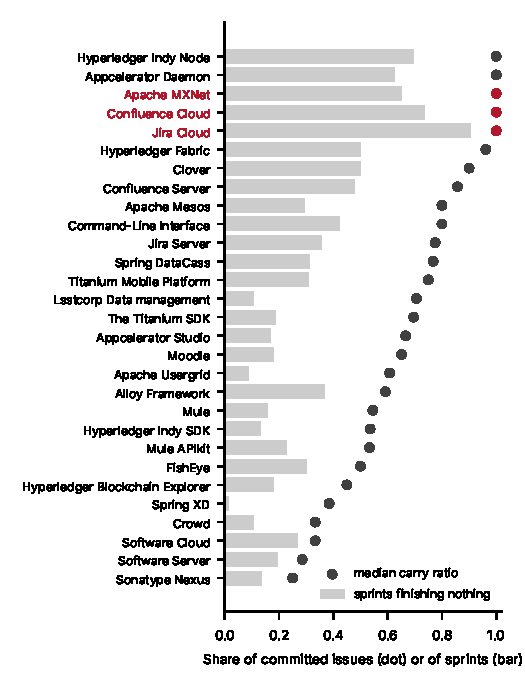
\includegraphics[width=\columnwidth]{fig_carry.pdf}
\caption{Per project, before the measurability check: median share of committed issues left unfinished at the planned end (dot) and share of sprints that finish none of their committed issues (bar). Red: the three projects where most sprint issues are closed without a resolution date.}
\label{fig:carry}
\end{figure}

The cohort is the remaining \NProj{} projects. After dropping each project's first sprint as a cold start, it has \NSprints{} sprints from \DateFrom{} to \DateTo, between \SprintMin{} and \SprintMax{} per project (median \SprintMed). Of these, \NNonempty{} commit at least one issue; we call them nonempty. Before the check, \FullNothingPct\% of nonempty sprints finished none of their committed issues; after it, \CleanNothingPct\%.

The outside set is the ten projects used in our earlier study: MariaDB MaxScale and ColumnStore, and eight MongoDB projects, exported from the organisations' public Jira and converted to the TAWOS layout. All ten pass the measurability check. They are used only for testing.

\subsection{Reconstruction}

For every sprint we replay the Sprint and Story Points fields of every issue back to the sprint's start and form the committed set (\ref{eq:committed}). Issues added later, issues removed later, and their story points at the start all come from the replay. Where an issue has no recorded story-point change, the replay falls back on the exported value; on average \FallbackMean\% of a sprint's committed issues are affected. Two custom fields are excluded from the replay: ``Actual Story Points'' in Spring XD, which is recorded after the work, and a retired duplicate in Moodle.

\emph{Reconstruction check.} No public record shows the board as it stood at each sprint start, so the replay cannot be compared with ground truth. It can, however, be checked for consistency, because replaying an issue's log forward must end in the values the export shows. For story points it does in \RecPointsAgree\% of the \RecPointsN{} issues with a story-point history. For the sprint field it does in \RecSprintAgree\% of the \RecSprintBoth{} issues where both the log and the export name a sprint of the cohort. For another \RecExportEmpty{} issues the export shows no sprint although the log's last event names one; the replay follows the log. Of the issues ever placed in a sprint, \RecHistoryPct\% have a sprint history; for the rest the replay has to take the exported sprint as the sprint at the start, the sprint-field counterpart of the story-point fallback. We repeat the main comparisons on projects where at least 85\% of such issues have a history (Section~\ref{sec:robust}).

\section{Outcomes, Features and Protocol}
\label{sec:protocol}

\subsection{Outcomes}

Table~\ref{tab:labels} lists the five outcomes. Late closure and spillover are carried over from our earlier work. The other three are new.

\emph{Serious spillover} is concerned with how much was left over rather than whether anything was. We fixed its primary threshold at a carry ratio of 30\% before seeing the full cohort. In hindsight this was a poor choice. The median nonempty sprint leaves \CarryMedPct\% of its committed issues unfinished, so the label is \PosSs\% positive, close to plain spillover (\PosSp\%). The median-based version (carry ratio above the training-set median, \PosSm\% positive), added after the development run, is better balanced. We keep the primary threshold as planned and report the median version beside it as a secondary result.

\emph{Seriously late} means the sprint was closed in Jira more than three days after its planned end (seven as a sensitivity check). Like late closure, it records an administrative event in the tracker.

\emph{Scope churn} means the issues added after the start and still in the sprint at its planned end make up at least 30\% of the committed count (50\% as a sensitivity check). It is defined only for sprints with five or more committed issues, and it is predicted at planning time only, because during the sprint the additions so far give the answer away.

\begin{table}[t]
\centering
\small
\caption{Outcomes, populations and positive rates (\NProj{} TAWOS projects). Nonempty: sprints that commit at least one issue. Indented rows are sensitivity versions.}
\label{tab:labels}
\begin{tabular}{@{}llrr@{}}
\toprule
Outcome & Population & Sprints & Positive \\
\midrule
Spillover & Nonempty & 2,409 & 90\% \\
Serious spillover & Nonempty & 2,409 & 82\% \\
Late closure & All & 3,676 & 41\% \\
Seriously late & All & 3,676 & 23\% \\
Scope churn & Nonempty, 5+ & 1,500 & 66\% \\
\quad Serious sp., median & same & 2,409 & 49\% \\
\quad Serious sp., 20\% & same & 2,409 & 86\% \\
\quad Serious sp., 50\% & same & 2,409 & 71\% \\
\quad Seriously late, 7 days & same & 3,676 & 13\% \\
\quad Scope churn, 50\% & same & 1,500 & 50\% \\
\bottomrule
\end{tabular}
\end{table}

\subsection{Feature sets}

Table~\ref{tab:families} lists the sets. Four of them are nested (scope within strict within strict+new within ours), so part of the benchmark is an ablation of one feature set. The two prior families, worki and choet, are partial versions that keep only what a public export supports. All features are admissible in the sense of Section~\ref{sec:theory}.

\begin{table}[t]
\centering
\small
\caption{Feature sets. Planning-time sets are scored at the sprint start; in-sprint sets at 25\% and 50\% of the planned duration. $^{\dagger}$: added after review.}
\label{tab:families}
\begin{tabular}{@{}p{1.6cm}p{6.3cm}@{}}
\toprule
Set & Contents \\
\midrule
scope & Committed issues, committed story points, sprint length. \\
strict & scope, parallel sprints, the last three finished sprints (completion ratio, carry-over, delivered points, completed and committed issues), scope relative to capacity, past lateness, and the project. \\
strict+new & strict and the four new features below. \\
choet & Iteration counts of \cite{choet2018} that the export supports: duration, issues and points at start, added and removed since start, done and to do at the checkpoint. \\
choet+ctx$^{\dagger}$ & choet and everything in strict+new, including the project. \\
worki & Burndown-shape indicators R1 to R11 after \cite{perez2024}, on issue counts. \\
ours & strict+new and 13 progress counts: elapsed share, days left, done and remaining issues and points, burn gap, required and observed rate, added and removed ratios. \\
ours+worki & ours and R1 to R11. \\
\bottomrule
\end{tabular}
\end{table}

The four \emph{new planning-time features} are: the share of committed issues that had been in another sprint before (carried in); the log of the median age of committed issues at the start; the share of committed issues with no estimate; and the share whose estimate was changed before the start (re-estimated).

The \emph{worki} set follows our reading of the verbal definitions in \cite{perez2024}, computed on the daily burndown of issue counts up to the checkpoint. Their study graded finished sprints using hours, whereas we score the same kind of indicator during the sprint using issue counts. Because the tasks differ, a large gap between ours and worki says little on its own. The more useful comparison is ours+worki minus ours, which asks whether burndown shape adds anything to progress counts. The \emph{choet} set leaves out what a public export cannot support, namely in-progress counts (there is no status history), team size and the Scrum master (the assignee is a final value), and all issue-level features. Ours differs from choet both in planning context (history, new features, project) and in its progress counts. The set choet+ctx separates the two. The difference choet+ctx minus choet measures what planning context adds to their counts, and ours minus choet+ctx measures what our progress counts add given the same context. Neither comparison is meant to rank the two studies.

\subsection{Models and protocol}

We use logistic regression with balanced class weights, a random forest \cite{breiman2001} (300 trees, depth 5) and histogram gradient boosting \cite{friedman2001} (depth 3, learning rate 0.05, 200 iterations), all from scikit-learn \cite{sklearn} with fixed settings and seed 42.

The \emph{primary analysis} uses gradient boosting on a per-project time split, with the first 70\% of each project's sprints by start date used for training and the rest for testing (\TestAll{} test sprints, \TestNonempty{} of them nonempty). For each outcome and comparison we report one paired AUC difference with two 95\% bootstrap intervals from 2,000 resamples. One resamples whole projects \cite{field2007} and serves as the test; the other resamples sprints. For the hypothesis comparisons we also report a two-sided bootstrap $p$-value from 10,000 project-level resamples and adjust it over all of them with Holm's method \cite{holm1979}. Because AUC can hide poor performance on a rare class \cite{davis2006}, we also report average precision for finding the minority class where the positive rate is high. All other analyses are secondary. They include the other two models, leave-one-project-out testing (no project feature), five time-ordered repeats, a tuned model, a single calendar cut-off in place of the per-project split, and the outside projects (trained on all of TAWOS, without the project feature and without story points, which MariaDB does not record). Decision thresholds come from Youden's index \cite{youden1950} on out-of-fold training scores, never from the test set.

\subsection{Hypotheses}

We wrote the study plan, the primary analysis and four hypotheses into a dated plan before the full-cohort run, and logged every later change with its reason. A hypothesis holds only where the project-level interval is above zero.
\begin{itemize}
\item \textbf{H1, new features} (strict+new minus strict, planning time): positive for scope churn and serious spillover, small and positive for spillover, about zero for the two late labels.
\item \textbf{H2, burndown shape} (ours minus worki, spillover labels): positive at both checkpoints.
\item \textbf{H3, planning context} (ours minus choet): positive and below 0.05 for every outcome.
\item \textbf{H4, new labels} (strict+new minus scope, planning time): positive for seriously late and scope churn, about zero for serious spillover.
\end{itemize}
The plan was written after a development run on eight projects. Of these, \DevProj{} remain in the cohort and hold \DevSprints{} of its sprints. The other \ConfProj{} had not been looked at when the hypotheses were written, so we repeat every hypothesis test on them alone, training and testing on those projects only, as a confirmation set. The measurability and reconstruction checks, the choet+ctx set, the Holm adjustment and the confirmation set were added after the full run, in response to review, and the plan logs them as such.

\section{Results}
\label{sec:results}

\subsection{Overview of the hypothesis tests}

Table~\ref{tab:hyp} and Fig.~\ref{fig:primary} give all \NHyp{} hypothesis comparisons. Of these, \NHoldRaw{} have a project-level interval above zero, \NHoldHolm{} survive the Holm adjustment, and \NHoldConf{} hold in both the full cohort and the confirmation set.

\begin{table*}[t]
\centering
\caption{All hypothesis comparisons (gradient boosting, per-project time split). $\Delta$: difference in AUC with its 95\% interval over projects. $p_{\mathrm{Holm}}$: bootstrap $p$-value from 10,000 project-level resamples, adjusted over the \NHyp{} comparisons. Confirmation: the same comparison trained and tested on the \ConfProj{} projects not used in the development run. $\checkmark$: interval above zero.}
\label{tab:hyp}
\begin{tabular}{@{}llrccc rc@{}}
\toprule
& & \multicolumn{4}{c}{\NProj{} projects} & \multicolumn{2}{c}{Confirmation} \\
\cmidrule(lr){3-6}\cmidrule(l){7-8}
& Outcome & $\Delta$ & 95\% interval & $p_{\mathrm{Holm}}$ & & $\Delta$ & \\
\midrule
H1 & Late closure & +0.001 & [$-$0.013, +0.012] & 0.975 &  & $-$0.009 &  \\
H1 & Seriously late & $-$0.006 & [$-$0.016, 0.000] & 0.628 &  & +0.002 &  \\
H1 & Spillover & +0.037 & [+0.022, +0.056] & 0.006 & $\checkmark$ & +0.016 &  \\
H1 & Serious spillover & +0.017 & [$-$0.008, +0.048] & 0.975 &  & +0.035 &  \\
H1 & Scope churn & +0.026 & [$-$0.028, +0.069] & 0.975 &  & +0.006 &  \\
\midrule
H2 & Spillover, 25\% & +0.131 & [+0.077, +0.196] & 0.002 & $\checkmark$ & +0.158 & $\checkmark$ \\
H2 & Spillover, 50\% & +0.194 & [+0.109, +0.272] & 0.002 & $\checkmark$ & +0.252 & $\checkmark$ \\
H2 & Serious spillover, 25\% & +0.179 & [+0.108, +0.256] & 0.002 & $\checkmark$ & +0.236 & $\checkmark$ \\
H2 & Serious spillover, 50\% & +0.178 & [+0.083, +0.261] & 0.006 & $\checkmark$ & +0.248 & $\checkmark$ \\
\midrule
H3 & Spillover, 25\% & +0.031 & [$-$0.002, +0.067] & 0.727 &  & +0.053 & $\checkmark$ \\
H3 & Spillover, 50\% & +0.034 & [0.000, +0.078] & 0.714 & $\checkmark$ & +0.081 & $\checkmark$ \\
H3 & Serious spillover, 25\% & +0.049 & [0.000, +0.111] & 0.662 &  & +0.111 & $\checkmark$ \\
H3 & Serious spillover, 50\% & +0.053 & [0.000, +0.117] & 0.648 &  & +0.099 & $\checkmark$ \\
H3 & Late closure, 25\% & +0.051 & [$-$0.010, +0.125] & 0.975 &  & +0.032 &  \\
H3 & Late closure, 50\% & +0.053 & [$-$0.013, +0.125] & 0.975 &  & +0.028 &  \\
H3 & Seriously late, 25\% & +0.067 & [$-$0.008, +0.138] & 0.937 &  & +0.073 & $\checkmark$ \\
H3 & Seriously late, 50\% & +0.093 & [+0.007, +0.193] & 0.622 & $\checkmark$ & +0.027 &  \\
\midrule
H4 & Late closure & +0.043 & [$-$0.013, +0.093] & 0.975 &  & +0.016 &  \\
H4 & Seriously late & +0.045 & [$-$0.020, +0.101] & 0.975 &  & +0.044 &  \\
H4 & Spillover & +0.034 & [$-$0.005, +0.082] & 0.975 &  & +0.089 & $\checkmark$ \\
H4 & Serious spillover & +0.088 & [+0.018, +0.161] & 0.223 & $\checkmark$ & +0.178 & $\checkmark$ \\
H4 & Scope churn & +0.063 & [$-$0.056, +0.207] & 0.975 &  & +0.065 &  \\
\bottomrule
\end{tabular}
\end{table*}

\begin{figure}[!htb]
\centering
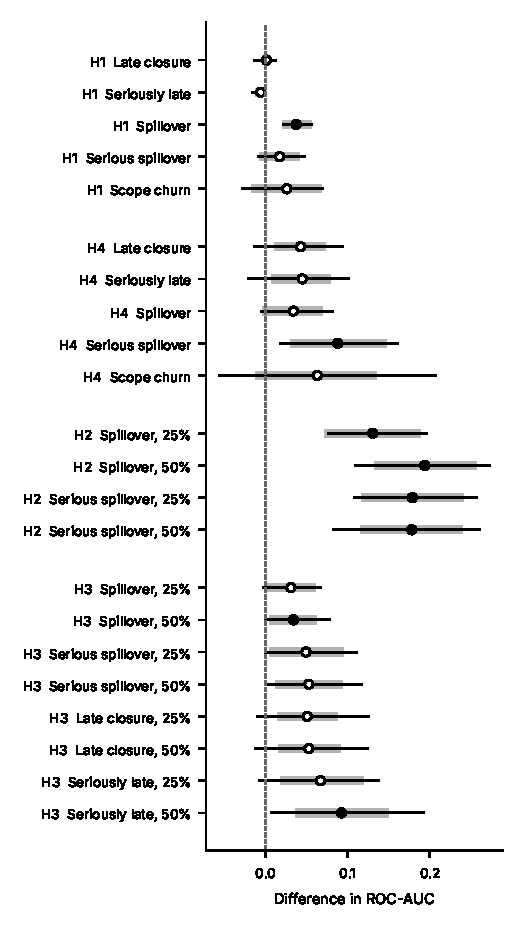
\includegraphics[width=\columnwidth]{fig_primary.pdf}
\caption{The hypothesis comparisons of Table~\ref{tab:hyp} on the full cohort. Dot: difference in AUC (filled where the project-level interval is above zero). Black line: 95\% interval over projects. Grey bar: 95\% interval over sprints.}
\label{fig:primary}
\end{figure}

\emph{H1 (new features).} The new features add \dPTNewSp{} \cPTNewSp{} for spillover, which survives the Holm adjustment, but only \dPCNewSp{} \cPCNewSp{} on the confirmation set. For serious spillover the gain is \dPTNewSs{} \cPTNewSs, with the same sign in all three models. For the two late labels it is about zero, as predicted. We read H1 as a small gain for spillover that we cannot confirm.

\emph{H2 (burndown shape).} H2 holds in every case. Ours beats worki by 0.13 to 0.19 AUC on both spillover labels at both checkpoints, in the full cohort and on the confirmation set. As explained in Section~\ref{sec:protocol}, the size of this gap says little by itself, and the fairer test is reported in Section~\ref{sec:fair}.

\emph{H3 (planning context).} Ours beats choet for every outcome, by 0.03 to 0.09, but on the full cohort the project-level interval clears zero clearly only for seriously late at 50\%; for the spillover labels it sits on zero. On the confirmation set the gain is larger and holds for both spillover labels. Section~\ref{sec:fair} examines where the gain comes from.

\emph{H4 (new labels).} This hypothesis failed where it was most specific. We predicted that history would add nothing to serious spillover beyond scope. It adds \dPTHistSs{} \cPTHistSs{} on the time split, \dPLHistSs{} \cPLHistSs{} under leave-one-project-out testing and \dPCHistSs{} on the confirmation set. It does not survive the Holm adjustment, but it holds under every other protocol and replicates on the confirmation set, so we regard it as the most robust result after H2. Seriously late and scope churn do not hold.

\subsection{Planning time}

Table~\ref{tab:planauc} gives the AUC of the planning-time sets. Late closure is hard to predict. Scope alone reaches \aPTLcScope, and the best set \aPTLcNew. The binomial model of Section~\ref{sec:theory} predicts that history should beat scope by more for serious spillover than for plain spillover, and this is what we observe. Strict minus scope is \dPTStrSp{} for spillover against \dPTStrSs{} for serious spillover on the time split, and \dPLStrSp{} against \dPLStrSs{} under leave-one-project-out testing. Plain spillover is mostly a matter of how many issues were committed, whereas serious spillover depends more on which team committed them. The median-based serious-spillover label shows the same pattern more clearly, with strict+new at \aPTSmNew{} against \aPTSmScope{} for scope.

\begin{table}[t]
\centering
\small
\caption{Planning-time ROC-AUC, gradient boosting. Time: per-project time split. LOPO: leave one project out (no project feature).}
\label{tab:planauc}
\setlength{\tabcolsep}{4pt}
\begin{tabular}{@{}lrrrrrr@{}}
\toprule
& \multicolumn{3}{c}{Time split} & \multicolumn{3}{c}{LOPO} \\
\cmidrule(lr){2-4}\cmidrule(l){5-7}
Outcome & scope & strict & +new & scope & strict & +new \\
\midrule
Spillover & 0.835 & 0.832 & 0.869 & 0.818 & 0.834 & 0.849 \\
Serious spillover & 0.681 & 0.752 & 0.769 & 0.609 & 0.723 & 0.748 \\
Late closure & 0.682 & 0.724 & 0.725 & 0.643 & 0.724 & 0.721 \\
Seriously late & 0.639 & 0.690 & 0.684 & 0.650 & 0.682 & 0.674 \\
Scope churn & 0.545 & 0.582 & 0.608 & 0.535 & 0.523 & 0.547 \\
\bottomrule
\end{tabular}
\end{table}

AUC is high for spillover partly because the label is \PosSp\% positive. Only \NegSp{} nonempty test sprints finish everything they committed (\NegSs{} for serious spillover). Average precision for finding those sprints (Table~\ref{tab:apneg} in the Appendix) is several times the base rate but well below one, so the spillover models are much better at confirming the common outcome than at spotting the rare good sprint.

\subsection{During the sprint}
\label{sec:fair}

Table~\ref{tab:inauc} gives the in-sprint AUC, on the nonempty sprints still open at the checkpoint (\InTestA{} test sprints at 25\%, \InTestB{} at 50\%). Table~\ref{tab:fair} gives the fair comparisons.

\begin{table}[t]
\centering
\small
\caption{In-sprint ROC-AUC at 25\% and 50\% of the planned duration, gradient boosting, time split.}
\label{tab:inauc}
\footnotesize
\setlength{\tabcolsep}{2.4pt}
\begin{tabular}{@{}llrrrrrr@{}}
\toprule
Outcome & At & scope & worki & choet & +ctx & ours & +worki \\
\midrule
Spillover & 25\% & 0.831 & 0.785 & 0.885 & 0.897 & 0.916 & 0.914 \\
 & 50\% & 0.834 & 0.743 & 0.903 & 0.910 & 0.937 & 0.937 \\
Serious spillover & 25\% & 0.695 & 0.665 & 0.794 & 0.828 & 0.843 & 0.841 \\
 & 50\% & 0.688 & 0.708 & 0.833 & 0.851 & 0.886 & 0.886 \\
Late closure & 25\% & 0.678 & 0.571 & 0.665 & 0.724 & 0.716 & 0.717 \\
 & 50\% & 0.676 & 0.634 & 0.679 & 0.742 & 0.731 & 0.736 \\
Seriously late & 25\% & 0.617 & 0.506 & 0.608 & 0.645 & 0.675 & 0.672 \\
 & 50\% & 0.605 & 0.537 & 0.594 & 0.693 & 0.686 & 0.680 \\
\bottomrule
\end{tabular}
\end{table}

\begin{table*}[t]
\centering
\footnotesize
\caption{What each family adds to the others during the sprint: differences in AUC with 95\% intervals over projects (gradient boosting, time split).}
\label{tab:fair}
\setlength{\tabcolsep}{4pt}
\begin{tabular}{@{}llccc@{}}
\toprule
Outcome & At & Burndown shape added & Planning context added & Our progress counts \\
& & ours+worki $-$ ours & choet+ctx $-$ choet & ours $-$ choet+ctx \\
\midrule
Spillover & 25\% & $-$0.002 [$-$0.006, +0.003] & +0.012 [$-$0.013, +0.043] & +0.018 [$-$0.008, +0.048] \\
 & 50\% & 0.000 [$-$0.006, +0.004] & +0.007 [$-$0.014, +0.032] & +0.027 [$-$0.004, +0.061] \\
Serious spillover & 25\% & $-$0.002 [$-$0.008, +0.004] & +0.034 [$-$0.011, +0.093] & +0.016 [$-$0.018, +0.048] \\
 & 50\% & 0.000 [$-$0.006, +0.005] & +0.018 [$-$0.021, +0.070] & +0.034 [+0.005, +0.069] \\
Late closure & 25\% & +0.001 [$-$0.009, +0.010] & +0.059 [$-$0.001, +0.125] & $-$0.008 [$-$0.022, +0.008] \\
 & 50\% & +0.004 [$-$0.003, +0.012] & +0.063 [$-$0.001, +0.135] & $-$0.011 [$-$0.023, +0.003] \\
Seriously late & 25\% & $-$0.003 [$-$0.014, +0.008] & +0.038 [$-$0.029, +0.105] & +0.029 [+0.002, +0.055] \\
 & 50\% & $-$0.007 [$-$0.018, +0.007] & +0.099 [+0.011, +0.192] & $-$0.006 [$-$0.042, +0.028] \\
\bottomrule
\end{tabular}
\end{table*}

\emph{Burndown shape.} Adding the worki set to ours changes AUC by at most \AddMax{} for any outcome at either checkpoint. On its own the worki set ranks worse than committed scope, with intervals below zero, for late closure at 25\% (\dITWsLcA{} \cITWsLcA), for seriously late at both checkpoints and for spillover at 50\%.

\emph{Planning context.} Added to the choet counts, planning context changes AUC by \dITCtxSpA{} and \dITCtxSpB{} for spillover and \dITCtxSsA{} and \dITCtxSsB{} for serious spillover; none of these intervals clears zero. Under leave-one-project-out testing it helps serious spillover (\dILCtxSsA{} \cILCtxSsA{} at 25\%). For seriously late at 50\% it adds \dITCtxSlB{} \cITCtxSlB.

\emph{Progress counts.} Our progress counts add a little beyond theirs for serious spillover at 50\% (\dITProgSsB{} \cITProgSsB), and on the confirmation set at both checkpoints. The H3 gap therefore comes partly from progress counts and partly from context, and neither part is large.

\emph{Outcomes.} Most of the in-sprint signal concerns the spillover labels. Serious spillover goes from \aPTSsNew{} at planning time to \aITSsAOurs{} at 25\% and \aITSsBOurs{} at 50\%. For late closure our set reaches only \aITLcAOurs{} and \aITLcBOurs, against \aITLcAScope{} and \aITLcBScope{} for scope alone on the same sprints.

\subsection{A binomial baseline without learning}

Table~\ref{tab:binomial} scores the binomial model of Section~\ref{sec:theory} as a predictor. For each sprint, $q_s$ is the pooled completion rate of the team's last three finished sprints known at the start, or the training-set rate where there is no history. Nothing else is fitted. Its AUC is \aBinSp{} against \aBinGbSp{} for gradient boosting on spillover (difference \dGbBinSp{} \cGbBinSp) and \aBinSs{} against \aBinGbSs{} on serious spillover (\dGbBinSs{} \cGbBinSs). The two cannot be distinguished statistically. For serious spillover the binomial model beats scope alone by \dBinScopeSs{} \cBinScopeSs. On the confirmation set the gap to gradient boosting is wider (\dGbBinCSp{} and \dGbBinCSs, intervals \cGbBinCSp{} and \cGbBinCSs) and the binomial model still beats scope for serious spillover (\dBinScopeCSs{} \cBinScopeCSs). This suggests that most of what the learned model adds over scope at planning time is an estimate of one number per team.

\begin{table}[t]
\centering
\small
\caption{The binomial model as a predictor on the nonempty test sprints. AUC and calibration slope (1 is ideal).}
\label{tab:binomial}
\setlength{\tabcolsep}{3pt}
\begin{tabular}{@{}lrrrr@{}}
\toprule
& \multicolumn{2}{c}{Spillover} & \multicolumn{2}{c}{Serious sp.} \\
\cmidrule(lr){2-3}\cmidrule(l){4-5}
Model & AUC & Slope & AUC & Slope \\
\midrule
Gradient boosting, scope & 0.835 & 0.89 & 0.681 & 0.88 \\
Binomial, no learning & 0.864 & 0.41 & 0.759 & 0.26 \\
Beta-binomial, one parameter & 0.854 & 0.59 & 0.745 & 0.49 \\
Gradient boosting, strict+new & 0.869 & 0.95 & 0.769 & 0.81 \\
\bottomrule
\end{tabular}
\end{table}

Its probabilities, however, are poorly calibrated. The calibration slopes are \sBinSp{} and \sBinSs, which means that the binomial model is overconfident. Table~\ref{tab:variance} in the Appendix suggests why. In every band of sprint size the observed variance of the carry ratio exceeds the binomial variance, by a factor of \VarRatioSmall{} for sprints of one to three issues and \VarRatioLarge{} for sprints of 16 or more. A gap that grows with sprint size is what Proposition~\ref{prop:overdisp} predicts when $r > 0$. The ratio of observed to binomial variance over the training sprints, the quantity behind Tarone's test of binomial fit \cite{tarone1979}, is \DispRatio, and the maximum-likelihood estimate is $r = \Rhat$ (likelihood-ratio statistic \LRstat{} against $r = 0$). The beta-binomial model matches the observed variance for large sprints (\VarBetaLarge{} against \VarObsLarge) and raises the slopes to \sBetaSp{} and \sBetaSs, at a small cost in ranking (\mBetaCostSp{} and \mBetaCostSs{} AUC). Neither is as well calibrated as gradient boosting (slopes \sGbSp{} and \sGbSs). Learning therefore matters mainly for well-calibrated probabilities and much less for ranking.

\subsection{What a warning is worth}

A difference of 0.03 AUC is hard for a team to interpret. Table~\ref{tab:budgets} in the Appendix therefore asks how many flagged sprints are real problems when a team can look into only 10\% or 20\% of its sprints. For serious spillover in its median form, the history-aware model raises the hit rate among the top 10\% from \bSmTenScope\% to \bSmTenNew\% (\bSmTenExtra{} more real problems among \bSmTenFlag{} flagged sprints), against a base rate of \bSmTenBase\%. For late closure the gain is \bLcTenScope\% to \bLcTenNew\%.

Table~\ref{tab:nb} applies the net benefit (\ref{eq:nb}) on the \NbN{} sprints scored at all three stages. Never warning scores zero. For serious spillover, warning on every sprint is almost as good as any model unless warnings are costly. At $p^{*} = 0.5$, warning on all sprints gives \nbSsHalfAll{} against \nbSsHalfPlan{} at planning and \nbSsHalfB{} at 50\%. Only at $p^{*} = 0.9$, where a warning must be nearly certain to pay, does the model clearly add value (\nbSsNinePlan{} at planning and \nbSsNineB{} at 50\%, against \nbSsNineAll{} for warning on all). There, waiting until 50\% of the sprint pays only if a warning at that point still averts at least \beSsNineB{} of what an early warning would. For late closure the picture is reversed. Warning on all sprints loses at any threshold above the base rate, the planning-time model gains a little (\nbLcThreePlan{} at $p^{*} = 0.3$, \nbLcHalfPlan{} at 0.5), and the in-sprint models gain no more than the planning model, so waiting never pays. Fig.~\ref{fig:reliability} shows the calibration behind these numbers.

\begin{table}[t]
\centering
\small
\caption{Net benefit (\ref{eq:nb}) per sprint, in units of the averted failure cost, on the same \NbN{} test sprints. All: warn on every sprint. Never warning scores 0.}
\label{tab:nb}
\setlength{\tabcolsep}{3pt}
\begin{tabular}{@{}lrrrrr@{}}
\toprule
Outcome & $p^{*}$ & All & Planning & 25\% & 50\% \\
\midrule
Serious spillover & 0.3 & +0.552 & +0.550 & +0.556 & +0.568 \\
Serious spillover & 0.5 & +0.352 & +0.353 & +0.369 & +0.380 \\
Serious spillover & 0.7 & +0.152 & +0.177 & +0.187 & +0.201 \\
Serious spillover & 0.9 & $-$0.048 & +0.022 & +0.037 & +0.042 \\
Late closure & 0.3 & +0.045 & +0.099 & +0.088 & +0.093 \\
Late closure & 0.5 & $-$0.155 & +0.032 & +0.032 & +0.033 \\
Late closure & 0.7 & $-$0.355 & $-$0.004 & $-$0.009 & $-$0.003 \\
Late closure & 0.9 & $-$0.555 & $-$0.002 & $-$0.003 & $-$0.004 \\
\bottomrule
\end{tabular}
\end{table}

\begin{figure}[!htb]
\centering
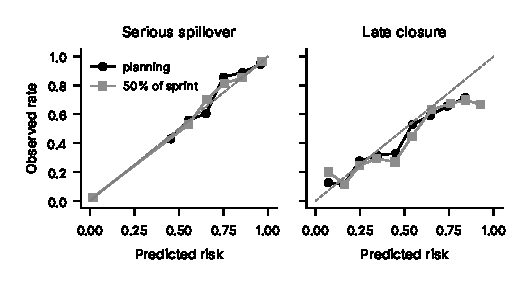
\includegraphics[width=\columnwidth]{fig_reliability.pdf}
\caption{Reliability of the gradient-boosting risk on the sprints of Table~\ref{tab:nb}: mean predicted risk against the observed rate, in bins of width 0.1 with at least ten sprints.}
\label{fig:reliability}
\end{figure}

\subsection{Outside projects}

Table~\ref{tab:external} trains on all of TAWOS and tests on each outside project with at least five sprints in each class. We find no evidence of transfer. For the two spillover labels, where history helped most inside TAWOS, scope alone scores \eSpScope{} and \eSsScope, and the history-aware sets score lower. For late closure all three sets sit between \eLcStrict{} and \eLcScope. Only \eKSp{} outside projects are testable for spillover, and the spread across projects is large, so the most we can say is that we found no sign of transfer. This is consistent with the reading in Section~\ref{sec:theory}, in which history features estimate one team's completion rate, an estimate that need not carry over to another organisation's teams.

\begin{table}[t]
\centering
\footnotesize
\caption{Outside projects: mean $\pm$ s.d.\ of per-project AUC, gradient boosting trained on all TAWOS sprints. $k$: projects with at least five sprints in each class.}
\label{tab:external}
\setlength{\tabcolsep}{3pt}
\begin{tabular}{@{}lrccc@{}}
\toprule
Outcome & $k$ & scope & strict & strict+new \\
\midrule
Spillover & 4 & 0.778 $\pm$ 0.138 & 0.759 $\pm$ 0.142 & 0.755 $\pm$ 0.152 \\
Serious spillover & 9 & 0.594 $\pm$ 0.122 & 0.559 $\pm$ 0.129 & 0.580 $\pm$ 0.110 \\
Late closure & 8 & 0.666 $\pm$ 0.144 & 0.641 $\pm$ 0.129 & 0.652 $\pm$ 0.104 \\
Seriously late & 8 & 0.564 $\pm$ 0.160 & 0.584 $\pm$ 0.211 & 0.606 $\pm$ 0.227 \\
Scope churn & 5 & 0.428 $\pm$ 0.209 & 0.596 $\pm$ 0.093 & 0.609 $\pm$ 0.140 \\
\bottomrule
\end{tabular}
\end{table}

\subsection{Robustness}
\label{sec:robust}

Table~\ref{tab:robust} in the Appendix repeats the main planning-time comparisons under five variants. \emph{Tuning.} With a small grid chosen on a time-ordered validation slice, the new features add \dPUNewSp{} \cPUNewSp{} for spillover and history beats scope for serious spillover by \dPUHistSs{} \cPUHistSs. With \emph{a single calendar cut} in early 2018 (training on sprints whose outcome was known before it and testing on sprints that start after it, \CutProj{} projects), the values are \dPKNewSp{} \cPKNewSp{} and \dPKHistSs{} \cPKHistSs. \emph{Without \RestrictedProj}, the two projects whose sprints mostly finish nothing although they pass the measurability check, they are \dPRNewSp{} \cPRNewSp{} and \dPRHistSs{} \cPRHistSs. \emph{Before the measurability check}, on all \NProjExport{} projects, the new features added more for serious spillover and less for spillover, which is why we report the check as a contribution. \emph{Sprint-history coverage.} On the \HistProj{} projects where at least 85\% of issues ever placed in a sprint have a sprint history, the new features add \dPHNewSp{} \cPHNewSp{} for spillover and history beats scope for serious spillover by \dPHHistSs{} \cPHHistSs. Burndown shape added to ours changes AUC by at most \HistAddMax, and planning context added to the choet counts gains more than on the full cohort (\dIHCtxSpA{} \cIHCtxSpA{} for spillover at 25\%), so the weak planning-context result may partly reflect missing sprint history rather than a weak signal. \emph{Story-point provenance.} On test sprints with no story-point fallback, the new features add \dPFNewSp{} \cPFNewSp{} for spillover and history beats scope for serious spillover by \dPFHistSs{} \cPFHistSs. The five time-ordered repeats agree with the time split (strict+new scores \repSp{} for spillover, \repSs{} for serious spillover and \repLc{} for late closure). Calibration is reported in Table~\ref{tab:calibration}, with slopes from \SlopeSpMin{} to \SlopeSpMax{} for the spillover labels and from \SlopeLateMin{} to \SlopeLateMax{} for the late labels, which are overconfident.

\section{Discussion}
\label{sec:discussion}

\subsection{Practical implications}

For teams, the results have three practical implications. During a sprint, simple progress counts (how much is done, how much is left and how fast work is being completed) carry nearly all of the signal, and their warnings for leftover work are reasonably well calibrated; burndown-shape indicators add little to them. Before a sprint starts, the team's own recent completion rate is the best guide to how much will be left over, and a team can use it directly through the binomial model, since the learned model and the new features add little to it. Finally, the models did not transfer between organisations in our data. A model trained on other organisations' teams did no better than a size rule, and a threshold carried from one team to another changes what a miss is worth (Proposition~\ref{prop:youden}). For outcomes as common as spillover, the decision analysis adds a further caution, since warning on every sprint is nearly as good as any model unless warnings are costly.

\subsection{Why lateness is hard}

Late closure records the moment someone pressed ``Complete sprint'' in Jira, which depends on meetings, holidays and habit as much as on the work itself. None of the feature families we tried improves its prediction much. We keep the label for continuity with earlier work, but we would not recommend building a tool on it. Seriously late is no easier to rank, and its scores are among the worst calibrated in the study.

\subsection{Threats to validity}
\label{sec:threats}

\emph{Construct.} The labels come from Jira fields, not from asking teams whether a sprint went badly. Late closure and seriously late measure when a sprint was closed in the tool. Spillover counts issues, not effort, and the measurability check catches only the recording problem it was designed for. A project that sets resolution dates late, for example at release, would pass it and still overstate spillover.

\emph{Internal.} The reconstruction depends on the change log. Where it is missing, story points fall back on the exported value; we measured the share and repeated the main comparisons without it. Issue type, priority and assignee are left out because only their final values exist, which also means the choet set lacks team and issue features its authors used. The strict, choet+ctx and ours sets carry the project as a feature; leave-one-project-out testing removes it.

\emph{Hypotheses and analysis choices.} The hypotheses were written after a development run on eight projects. Several choices were made after the full run, namely the measurability check, the choet+ctx set, the Holm adjustment, the confirmation set, the tuned and calendar-cut variants and the decision analysis. All are logged with dates and reasons, and we report their effect whichever way it went. The confirmation set is our main answer to this threat. The in-sprint and serious-spillover results hold there, whereas the new-features result does not.

\emph{Conclusion.} The project-level interval resamples only \NProj{} clusters, so it is wide. We treat a result as holding only when the project interval clears zero, and report the adjusted values beside it.

\emph{External.} All projects are open source, and a handful of organisations contribute most TAWOS projects. The outside test covers two more organisations and ten projects, few of which have enough sprints in both classes for every label.

\section{Conclusion}

Under one leakage-aware protocol, and after checking that the outcomes can be measured, the kinds of signal used in the sprint-risk literature differ considerably. Progress counts dominate during a sprint and burndown shape adds little, while team history explains how much work is left over but not when the sprint is closed. In our data, nothing learned from one organisation's history helped another's. The formal setting turns these observations into results that can be checked. Empty sprints inflate AUC by an exact amount, a fitted threshold carries a hidden cost ratio, the choice between ``any'' and ``serious'' spillover determines whether history can matter, and correlated issue completion explains why a model with no learning ranks well but gives poorly calibrated probabilities. A natural next step is to ask teams whether the sprints these models flag are the ones they would have wanted to hear about.

\section*{Data Availability}

Code, export queries, the measurability and reconstruction checks, the reconstructed frames, every result file and the dated study plan with its change log are at \url{https://github.com/hani-ziad/journal-ieee-access-2027}. TAWOS \cite{tawos} is released under the Apache License 2.0 for research use, and the repository includes the extract we used. The outside projects' issues come from the public Jira sites of MariaDB and MongoDB; we do not redistribute them, but the repository includes the scripts that pull and convert them.

\appendix

\section*{Appendix: Further Results}

\begin{table}[h]
\centering
\small
\caption{Variance of the carry ratio around $1 - \hat q_s$ on the training sprints, by committed issues: observed, binomial (\ref{eq:ratio}) and beta-binomial (\ref{eq:overdisp}) with $r = \Rhat$.}
\label{tab:variance}
\begin{tabular}{@{}lrrrr@{}}
\toprule
Issues & Sprints & Observed & Binomial & Beta-bin. \\
\midrule
1--3 & 471 & 0.201 & 0.120 & 0.132 \\
4--7 & 373 & 0.094 & 0.038 & 0.064 \\
8--15 & 396 & 0.064 & 0.017 & 0.047 \\
16+ & 435 & 0.044 & 0.008 & 0.041 \\
\bottomrule
\end{tabular}
\end{table}

\begin{table}[h]
\centering
\small
\caption{Warning budgets at planning time: share of flagged sprints that are real problems (\%) when the top 10\% or 20\% of test sprints by risk are flagged. Base: positive rate.}
\label{tab:budgets}
\setlength{\tabcolsep}{3pt}
\begin{tabular}{@{}lrrrrr@{}}
\toprule
Outcome & Flag & Base & scope & strict & +new \\
\midrule
Serious sp. (median) & 10\% & 57 & 75 & 78 & 81 \\
 & 20\% & 57 & 68 & 71 & 75 \\
Late closure & 10\% & 35 & 62 & 64 & 63 \\
 & 20\% & 35 & 65 & 64 & 63 \\
\bottomrule
\end{tabular}
\end{table}

\begin{table}[h]
\centering
\small
\caption{Average precision for finding the sprints that do \emph{not} spill (planning time, gradient boosting, time split). Base: share of such sprints among the nonempty test sprints.}
\label{tab:apneg}
\setlength{\tabcolsep}{3pt}
\begin{tabular}{@{}lrrrrr@{}}
\toprule
Outcome & $n$ & Base & scope & strict & +new \\
\midrule
Spillover & 73 & 0.099 & 0.378 & 0.464 & 0.499 \\
Serious spillover & 110 & 0.150 & 0.315 & 0.407 & 0.400 \\
\bottomrule
\end{tabular}
\end{table}

\begin{table}[h]
\centering
\footnotesize
\caption{Main planning-time differences in AUC under each robustness variant. Columns: new features (strict+new $-$ strict) and history over scope (strict+new $-$ scope) for spillover (Sp), serious spillover (Ss) and late closure (Lc). $^{*}$: project-level interval above zero.}
\label{tab:robust}
\scriptsize
\setlength{\tabcolsep}{2pt}
\begin{tabular}{@{}lrrrrrr@{}}
\toprule
& \multicolumn{3}{c}{New features} & \multicolumn{3}{c}{History over scope} \\
\cmidrule(lr){2-4}\cmidrule(l){5-7}
Variant & Sp & Ss & Lc & Sp & Ss & Lc \\
\midrule
Primary & +0.037$^{*}$ & +0.017 & +0.001 & +0.034 & +0.088$^{*}$ & +0.043 \\
Tuned & +0.028$^{*}$ & +0.024$^{*}$ & $-$0.002 & +0.027$^{*}$ & +0.081$^{*}$ & +0.021 \\
Calendar cut & +0.035$^{*}$ & +0.021 & $-$0.003 & +0.053$^{*}$ & +0.079$^{*}$ & +0.032 \\
Without 2 projects & +0.038$^{*}$ & +0.018 & +0.001 & +0.031 & +0.071$^{*}$ & +0.042 \\
Uncleaned (29) & +0.028$^{*}$ & +0.026$^{*}$ & $-$0.006 & +0.040$^{*}$ & +0.104$^{*}$ & +0.011 \\
\bottomrule
\end{tabular}
\end{table}

\begin{table}[h]
\centering
\small
\caption{Calibration on the time-split test set, gradient boosting. Ref.: Brier score of the test prevalence. ECE: expected calibration error, ten bins.}
\label{tab:calibration}
\setlength{\tabcolsep}{3.5pt}
\begin{tabular}{@{}llrrrr@{}}
\toprule
Outcome & Stage & Brier & Ref. & ECE & Slope \\
\midrule
Spillover & planning & 0.066 & 0.090 & 0.028 & 0.95 \\
 & in-sprint 25\% & 0.053 & 0.090 & 0.014 & 0.97 \\
 & in-sprint 50\% & 0.043 & 0.089 & 0.010 & 0.95 \\
Serious spillover & planning & 0.109 & 0.127 & 0.036 & 0.81 \\
 & in-sprint 25\% & 0.089 & 0.127 & 0.020 & 0.87 \\
 & in-sprint 50\% & 0.070 & 0.126 & 0.013 & 0.93 \\
Late closure & planning & 0.198 & 0.226 & 0.060 & 0.79 \\
 & in-sprint 25\% & 0.200 & 0.225 & 0.059 & 0.73 \\
 & in-sprint 50\% & 0.196 & 0.226 & 0.069 & 0.78 \\
Seriously late & planning & 0.147 & 0.155 & 0.055 & 0.68 \\
 & in-sprint 25\% & 0.139 & 0.146 & 0.050 & 0.69 \\
 & in-sprint 50\% & 0.140 & 0.147 & 0.026 & 0.70 \\
\bottomrule
\end{tabular}
\end{table}

\section*{Acknowledgment}
%% IEEE Access requires AI-generated text to be disclosed here, with a citation to the AI system in the
%% sections that use it. Edit this paragraph so it says exactly how AI was used, or delete it if it was not.
The author used an AI assistant (Claude, Anthropic) to help draft and edit parts of the text and the
analysis code. The author checked every statement, number and reference and takes full responsibility
for the content.

\begin{thebibliography}{99}

\bibitem{choet2018} M. Choetkiertikul, H. K. Dam, T. Tran, A. Ghose, and J. Grundy, ``Predicting delivery capability in iterative software development,'' \emph{IEEE Trans. Softw. Eng.}, vol. 44, no. 6, pp. 551--573, Jun. 2018, doi: \url{10.1109/TSE.2017.2693989}.

\bibitem{sprint2vec} M. Choetkiertikul, P. Banyongrakkul, C. Ragkhitwetsagul, S. Tuarob, H. K. Dam, and T. Sunetnanta, ``Sprint2Vec: A deep characterization of sprints in iterative software development,'' \emph{IEEE Trans. Softw. Eng.}, vol. 51, no. 1, pp. 220--242, Jan. 2025, doi: \url{10.1109/TSE.2024.3509016}.

\bibitem{hearty2009} P. Hearty, N. Fenton, D. Marquez, and M. Neil, ``Predicting project velocity in XP using a learning dynamic Bayesian network model,'' \emph{IEEE Trans. Softw. Eng.}, vol. 35, no. 1, pp. 124--137, Jan. 2009, doi: \url{10.1109/TSE.2008.76}.

\bibitem{perez2024} Y. J. P\'erez Castillo, S. D. Orantes Jim\'enez, and P. O. Letelier Torres, ``Sprint management in Agile approach: Progress and velocity evaluation applying machine learning,'' \emph{Information}, vol. 15, no. 11, Art. no. 726, 2024, doi: \url{10.3390/info15110726}.

\bibitem{obike2025} P. G. Obike, V. E. Ekong, and O. U. Obot, ``A novel scoring-based Agile sprint deliverability prediction and prioritization using machine learning,'' \emph{Int. J. Comput. Appl.}, vol. 187, no. 49, pp. 40--53, 2025, doi: \url{10.5120/ijca2025925837}.

\bibitem{kula2022} E. Kula, E. Greuter, A. van Deursen, and G. Gousios, ``Factors affecting on-time delivery in large-scale agile software development,'' \emph{IEEE Trans. Softw. Eng.}, vol. 48, no. 9, pp. 3573--3592, Sep. 2022, doi: \url{10.1109/TSE.2021.3101192}.

\bibitem{kaufman2012} S. Kaufman, S. Rosset, C. Perlich, and O. Stitelman, ``Leakage in data mining: Formulation, detection, and avoidance,'' \emph{ACM Trans. Knowl. Discov. Data}, vol. 6, no. 4, pp. 1--21, 2012, doi: \url{10.1145/2382577.2382579}.

\bibitem{kapoor2023} S. Kapoor and A. Narayanan, ``Leakage and the reproducibility crisis in machine-learning-based science,'' \emph{Patterns}, vol. 4, no. 9, Art. no. 100804, 2023, doi: \url{10.1016/j.patter.2023.100804}.

\bibitem{abusharkh2027} H. AbuSharkh, M. Hanif, and R. Damseh, ``Reconstructing sprint-start Jira state for leakage-aware outcome prediction,'' submitted to the IEEE Canadian Conf. Electr. Comput. Eng. (CCECE), 2027.

\bibitem{tawos} V. Tawosi, A. Al-Subaihin, R. Moussa, and F. Sarro, ``A versatile dataset of agile open source software projects,'' in \emph{Proc. 19th Int. Conf. Mining Softw. Repositories (MSR)}, 2022, pp. 707--711, doi: \url{10.1145/3524842.3528029}.

\bibitem{choet2015} M. Choetkiertikul, H. K. Dam, T. Tran, and A. Ghose, ``Characterization and prediction of issue-related risks in software projects,'' in \emph{Proc. IEEE/ACM 12th Working Conf. Mining Softw. Repositories (MSR)}, 2015, pp. 280--291, doi: \url{10.1109/MSR.2015.33}.

\bibitem{choet2017} M. Choetkiertikul, H. K. Dam, T. Tran, and A. Ghose, ``Predicting the delay of issues with due dates in software projects,'' \emph{Empir. Softw. Eng.}, vol. 22, no. 3, pp. 1223--1263, 2017, doi: \url{10.1007/s10664-016-9496-7}.

\bibitem{kula2021} E. Kula, A. van Deursen, and G. Gousios, ``Modeling team dynamics for the characterization and prediction of delays in user stories,'' in \emph{Proc. 36th IEEE/ACM Int. Conf. Automated Softw. Eng. (ASE)}, 2021, pp. 991--1002, doi: \url{10.1109/ASE51524.2021.9678939}.

\bibitem{choet2019} M. Choetkiertikul, H. K. Dam, T. Tran, T. Pham, A. Ghose, and T. Menzies, ``A deep learning model for estimating story points,'' \emph{IEEE Trans. Softw. Eng.}, vol. 45, no. 7, pp. 637--656, Jul. 2019, doi: \url{10.1109/TSE.2018.2792473}.

\bibitem{porru2016} S. Porru, A. Murgia, S. Demeyer, M. Marchesi, and R. Tonelli, ``Estimating story points from issue reports,'' in \emph{Proc. 12th Int. Conf. Predictive Models Data Analytics Softw. Eng. (PROMISE)}, 2016, pp. 1--10, doi: \url{10.1145/2972958.2972959}.

\bibitem{fu2023} M. Fu and C. Tantithamthavorn, ``GPT2SP: A transformer-based agile story point estimation approach,'' \emph{IEEE Trans. Softw. Eng.}, vol. 49, no. 2, pp. 611--625, Feb. 2023, doi: \url{10.1109/TSE.2022.3158252}.

\bibitem{tawosi2023} V. Tawosi, R. Moussa, and F. Sarro, ``Agile effort estimation: Have we solved the problem yet? Insights from a replication study,'' \emph{IEEE Trans. Softw. Eng.}, vol. 49, no. 4, pp. 2677--2697, Apr. 2023, doi: \url{10.1109/TSE.2022.3228739}.

\bibitem{ortu2015} M. Ortu, G. Destefanis, B. Adams, A. Murgia, M. Marchesi, and R. Tonelli, ``The JIRA repository dataset: Understanding social aspects of software development,'' in \emph{Proc. 11th Int. Conf. Predictive Models Data Analytics Softw. Eng. (PROMISE)}, 2015, pp. 1--4, doi: \url{10.1145/2810146.2810147}.

\bibitem{montgomery2022} L. Montgomery, C. L\"uders, and W. Maalej, ``An alternative issue tracking dataset of public Jira repositories,'' in \emph{Proc. 19th Int. Conf. Mining Softw. Repositories (MSR)}, 2022, pp. 73--77, doi: \url{10.1145/3524842.3528486}.

\bibitem{tanti2017} C. Tantithamthavorn, S. McIntosh, A. E. Hassan, and K. Matsumoto, ``An empirical comparison of model validation techniques for defect prediction models,'' \emph{IEEE Trans. Softw. Eng.}, vol. 43, no. 1, pp. 1--18, Jan. 2017, doi: \url{10.1109/TSE.2016.2584050}.

\bibitem{bangash2020} A. A. Bangash, H. Sahar, A. Hindle, and K. Ali, ``On the time-based conclusion stability of cross-project defect prediction models,'' \emph{Empir. Softw. Eng.}, vol. 25, no. 6, pp. 5047--5083, 2020, doi: \url{10.1007/s10664-020-09878-9}.

\bibitem{falessi2020} D. Falessi, J. Huang, L. Narayana, J. F. Thai, and B. Turhan, ``On the need of preserving order of data when validating within-project defect classifiers,'' \emph{Empir. Softw. Eng.}, vol. 25, no. 6, pp. 4805--4830, 2020, doi: \url{10.1007/s10664-020-09868-x}.

\bibitem{jimenez2019} M. Jimenez, R. Rwemalika, M. Papadakis, F. Sarro, Y. Le Traon, and M. Harman, ``The importance of accounting for real-world labelling when predicting software vulnerabilities,'' in \emph{Proc. 27th ACM Joint Meeting Eur. Softw. Eng. Conf. Symp. Found. Softw. Eng. (ESEC/FSE)}, 2019, pp. 695--705, doi: \url{10.1145/3338906.3338941}.

\bibitem{shepperd2014} M. Shepperd, D. Bowes, and T. Hall, ``Researcher bias: The use of machine learning in software defect prediction,'' \emph{IEEE Trans. Softw. Eng.}, vol. 40, no. 6, pp. 603--616, Jun. 2014, doi: \url{10.1109/TSE.2014.2322358}.

\bibitem{marquez2018} A. E. M\'arquez-Chamorro, M. Resinas, and A. Ruiz-Cort\'es, ``Predictive monitoring of business processes: A survey,'' \emph{IEEE Trans. Serv. Comput.}, vol. 11, no. 6, pp. 962--977, 2018, doi: \url{10.1109/TSC.2017.2772256}.

\bibitem{teinemaa2019} I. Teinemaa, M. Dumas, M. La Rosa, and F. M. Maggi, ``Outcome-oriented predictive process monitoring: Review and benchmark,'' \emph{ACM Trans. Knowl. Discov. Data}, vol. 13, no. 2, pp. 1--57, 2019, doi: \url{10.1145/3301300}.

\bibitem{difrancesco2018} C. Di Francescomarino, C. Ghidini, F. M. Maggi, and F. Milani, ``Predictive process monitoring methods: Which one suits me best?'' in \emph{Business Process Management (BPM)}, Lecture Notes in Computer Science, 2018, pp. 462--479, doi: \url{10.1007/978-3-319-98648-7_27}.

\bibitem{fahrenkrog2022} S. A. Fahrenkrog-Petersen, N. Tax, I. Teinemaa, M. Dumas, M. de Leoni, F. M. Maggi, and M. Weidlich, ``Fire now, fire later: Alarm-based systems for prescriptive process monitoring,'' \emph{Knowl. Inf. Syst.}, vol. 64, no. 2, pp. 559--587, 2022, doi: \url{10.1007/s10115-021-01633-w}.

\bibitem{fawcett2006} T. Fawcett, ``An introduction to ROC analysis,'' \emph{Pattern Recognit. Lett.}, vol. 27, no. 8, pp. 861--874, 2006, doi: \url{10.1016/j.patrec.2005.10.010}.

\bibitem{hand2009} D. J. Hand, ``Measuring classifier performance: A coherent alternative to the area under the ROC curve,'' \emph{Mach. Learn.}, vol. 77, no. 1, pp. 103--123, 2009, doi: \url{10.1007/s10994-009-5119-5}.

\bibitem{hernandez2012} J. Hern\'andez-Orallo, P. Flach, and C. Ferri, ``A unified view of performance metrics: Translating threshold choice into expected classification loss,'' \emph{J. Mach. Learn. Res.}, vol. 13, no. 91, pp. 2813--2869, 2012.

\bibitem{elkan2001} C. Elkan, ``The foundations of cost-sensitive learning,'' in \emph{Proc. 17th Int. Joint Conf. Artif. Intell. (IJCAI)}, 2001, pp. 973--978.

\bibitem{brier1950} G. W. Brier, ``Verification of forecasts expressed in terms of probability,'' \emph{Monthly Weather Rev.}, vol. 78, no. 1, pp. 1--3, 1950, doi: \url{10.1175/1520-0493(1950)078<0001:VOFEIT>2.0.CO;2}.

\bibitem{vancalster2019} B. Van Calster, D. J. McLernon, M. van Smeden, L. Wynants, and E. W. Steyerberg, ``Calibration: The Achilles heel of predictive analytics,'' \emph{BMC Med.}, vol. 17, 2019, doi: \url{10.1186/s12916-019-1466-7}.

\bibitem{niculescu2005} A. Niculescu-Mizil and R. Caruana, ``Predicting good probabilities with supervised learning,'' in \emph{Proc. 22nd Int. Conf. Mach. Learn. (ICML)}, 2005, pp. 625--632, doi: \url{10.1145/1102351.1102430}.

\bibitem{skellam1948} J. G. Skellam, ``A probability distribution derived from the binomial distribution by regarding the probability of success as variable between the sets of trials,'' \emph{J. R. Stat. Soc. Ser. B}, vol. 10, no. 2, pp. 257--261, 1948, doi: \url{10.1111/j.2517-6161.1948.tb00014.x}.

\bibitem{vickers2006} A. J. Vickers and E. B. Elkin, ``Decision curve analysis: A novel method for evaluating prediction models,'' \emph{Med. Decis. Making}, vol. 26, no. 6, pp. 565--574, 2006, doi: \url{10.1177/0272989X06295361}.

\bibitem{breiman2001} L. Breiman, ``Random forests,'' \emph{Mach. Learn.}, vol. 45, no. 1, pp. 5--32, 2001, doi: \url{10.1023/A:1010933404324}.

\bibitem{friedman2001} J. H. Friedman, ``Greedy function approximation: A gradient boosting machine,'' \emph{Ann. Statist.}, vol. 29, no. 5, pp. 1189--1232, 2001, doi: \url{10.1214/aos/1013203451}.

\bibitem{sklearn} F. Pedregosa \emph{et al.}, ``Scikit-learn: Machine learning in Python,'' \emph{J. Mach. Learn. Res.}, vol. 12, no. 85, pp. 2825--2830, 2011.

\bibitem{field2007} C. A. Field and A. H. Welsh, ``Bootstrapping clustered data,'' \emph{J. R. Stat. Soc. Ser. B}, vol. 69, no. 3, pp. 369--390, 2007, doi: \url{10.1111/j.1467-9868.2007.00593.x}.

\bibitem{holm1979} S. Holm, ``A simple sequentially rejective multiple test procedure,'' \emph{Scand. J. Statist.}, vol. 6, no. 2, pp. 65--70, 1979.

\bibitem{davis2006} J. Davis and M. Goadrich, ``The relationship between precision-recall and ROC curves,'' in \emph{Proc. 23rd Int. Conf. Mach. Learn. (ICML)}, 2006, pp. 233--240, doi: \url{10.1145/1143844.1143874}.

\bibitem{youden1950} W. J. Youden, ``Index for rating diagnostic tests,'' \emph{Cancer}, vol. 3, no. 1, pp. 32--35, 1950, doi: \url{10.1002/1097-0142(1950)3:1<32::AID-CNCR2820030106>3.0.CO;2-3}.

\bibitem{tarone1979} R. E. Tarone, ``Testing the goodness of fit of the binomial distribution,'' \emph{Biometrika}, vol. 66, no. 3, pp. 585--590, 1979, doi: \url{10.1093/biomet/66.3.585}.

\end{thebibliography}

\begin{IEEEbiography}[{
\includegraphics[width=1in,height=1.25in,clip,keepaspectratio]{hani_abusharkh.jpg}}]{Hani AbuSharkh}
received the M.A.Sc. degree in information systems technology from Concordia University, Montreal, QC,
Canada, in 2011. He is currently pursuing the Ph.D. degree in informatics and computing at United Arab
Emirates University, Al Ain, United Arab Emirates. He is a Lecturer in Computer Science at the Higher
Colleges of Technology, United Arab Emirates. He previously
taught computer science for three years at Vanier College, Montreal, Canada. Before teaching, he worked for
more than ten years as a software engineer in the technology, automotive, aviation, defence and
secure-payments sectors, with organizations including Ford Motor Company, General Electric, Thales,
Lockheed Martin and Apple, on embedded and real-time systems, secure payment
technology and cybersecurity. He holds four Scrum certifications, CSM, A-CSM, CS-CSM and Scrum for AI.
His research interests include agile software development, mining software repositories and machine
learning for software project management.
\end{IEEEbiography}

\EOD

\end{document}
